\documentclass[twoside]{book}

% Packages required by doxygen
\usepackage{fixltx2e}
\usepackage{calc}
\usepackage{doxygen}
\usepackage[export]{adjustbox} % also loads graphicx
\usepackage{graphicx}
\usepackage[utf8]{inputenc}
\usepackage{makeidx}
\usepackage{multicol}
\usepackage{multirow}
\PassOptionsToPackage{warn}{textcomp}
\usepackage{textcomp}
\usepackage[nointegrals]{wasysym}
\usepackage[table]{xcolor}

% Font selection
\usepackage[T1]{fontenc}
\usepackage[scaled=.90]{helvet}
\usepackage{courier}
\usepackage{amssymb}
\usepackage{sectsty}
\renewcommand{\familydefault}{\sfdefault}
\allsectionsfont{%
  \fontseries{bc}\selectfont%
  \color{darkgray}%
}
\renewcommand{\DoxyLabelFont}{%
  \fontseries{bc}\selectfont%
  \color{darkgray}%
}
\newcommand{\+}{\discretionary{\mbox{\scriptsize$\hookleftarrow$}}{}{}}

% Page & text layout
\usepackage{geometry}
\geometry{%
  a4paper,%
  top=2.5cm,%
  bottom=2.5cm,%
  left=2.5cm,%
  right=2.5cm%
}
\tolerance=750
\hfuzz=15pt
\hbadness=750
\setlength{\emergencystretch}{15pt}
\setlength{\parindent}{0cm}
\setlength{\parskip}{3ex plus 2ex minus 2ex}
\makeatletter
\renewcommand{\paragraph}{%
  \@startsection{paragraph}{4}{0ex}{-1.0ex}{1.0ex}{%
    \normalfont\normalsize\bfseries\SS@parafont%
  }%
}
\renewcommand{\subparagraph}{%
  \@startsection{subparagraph}{5}{0ex}{-1.0ex}{1.0ex}{%
    \normalfont\normalsize\bfseries\SS@subparafont%
  }%
}
\makeatother

% Headers & footers
\usepackage{fancyhdr}
\pagestyle{fancyplain}
\fancyhead[LE]{\fancyplain{}{\bfseries\thepage}}
\fancyhead[CE]{\fancyplain{}{}}
\fancyhead[RE]{\fancyplain{}{\bfseries\leftmark}}
\fancyhead[LO]{\fancyplain{}{\bfseries\rightmark}}
\fancyhead[CO]{\fancyplain{}{}}
\fancyhead[RO]{\fancyplain{}{\bfseries\thepage}}
\fancyfoot[LE]{\fancyplain{}{}}
\fancyfoot[CE]{\fancyplain{}{}}
\fancyfoot[RE]{\fancyplain{}{\bfseries\scriptsize Generated by Doxygen }}
\fancyfoot[LO]{\fancyplain{}{\bfseries\scriptsize Generated by Doxygen }}
\fancyfoot[CO]{\fancyplain{}{}}
\fancyfoot[RO]{\fancyplain{}{}}
\renewcommand{\footrulewidth}{0.4pt}
\renewcommand{\chaptermark}[1]{%
  \markboth{#1}{}%
}
\renewcommand{\sectionmark}[1]{%
  \markright{\thesection\ #1}%
}

% Indices & bibliography
\usepackage{natbib}
\usepackage[titles]{tocloft}
\setcounter{tocdepth}{3}
\setcounter{secnumdepth}{5}
\makeindex

% Hyperlinks (required, but should be loaded last)
\usepackage{ifpdf}
\ifpdf
  \usepackage[pdftex,pagebackref=true]{hyperref}
\else
  \usepackage[ps2pdf,pagebackref=true]{hyperref}
\fi
\hypersetup{%
  colorlinks=true,%
  linkcolor=blue,%
  citecolor=blue,%
  unicode%
}

% Custom commands
\newcommand{\clearemptydoublepage}{%
  \newpage{\pagestyle{empty}\cleardoublepage}%
}

\usepackage{caption}
\captionsetup{labelsep=space,justification=centering,font={bf},singlelinecheck=off,skip=4pt,position=top}

%===== C O N T E N T S =====

\begin{document}

% Titlepage & ToC
\hypersetup{pageanchor=false,
             bookmarksnumbered=true,
             pdfencoding=unicode
            }
\pagenumbering{alph}
\begin{titlepage}
\vspace*{7cm}
\begin{center}%
{\Large X\+N\+LO -\/ U\+P\+PE \\[1ex]\large 1.\+3.\+0 }\\
\vspace*{1cm}
{\large Generated by Doxygen 1.8.13}\\
\end{center}
\end{titlepage}
\clearemptydoublepage
\pagenumbering{roman}
\tableofcontents
\clearemptydoublepage
\pagenumbering{arabic}
\hypersetup{pageanchor=true}

%--- Begin generated contents ---
\chapter{Namespace Index}
\section{Namespace List}
Here is a list of all namespaces with brief descriptions\+:\begin{DoxyCompactList}
\item\contentsline{section}{\mbox{\hyperlink{namespace_h_h}{HH}} }{\pageref{namespace_h_h}}{}
\item\contentsline{section}{\mbox{\hyperlink{namespace_x_n_l_o}{X\+N\+LO}} }{\pageref{namespace_x_n_l_o}}{}
\end{DoxyCompactList}

\chapter{Class Index}
\section{Class List}
Here are the classes, structs, unions and interfaces with brief descriptions\+:\begin{DoxyCompactList}
\item\contentsline{section}{\hyperlink{class_h_h_1_1_config___settings}{H\+H\+::\+Config\+\_\+\+Settings} }{\pageref{class_h_h_1_1_config___settings}}{}
\item\contentsline{section}{\hyperlink{structdetect}{detect$<$ typename, class, typename $>$} }{\pageref{structdetect}}{}
\item\contentsline{section}{\hyperlink{structdetect_3_01_t_00_01_op_00_01void__t_3_01_op_3_01_t_01_4_01_4_01_4}{detect$<$ T, Op, void\+\_\+t$<$ Op$<$ T $>$ $>$ $>$} }{\pageref{structdetect_3_01_t_00_01_op_00_01void__t_3_01_op_3_01_t_01_4_01_4_01_4}}{}
\item\contentsline{section}{\hyperlink{class_d_h_t}{D\+HT} }{\pageref{class_d_h_t}}{}
\item\contentsline{section}{\hyperlink{classgrid__rkr}{grid\+\_\+rkr} }{\pageref{classgrid__rkr}}{}
\item\contentsline{section}{\hyperlink{classgrid__tw}{grid\+\_\+tw} }{\pageref{classgrid__tw}}{}
\item\contentsline{section}{\hyperlink{class_x_n_l_o_1_1grid__tw}{X\+N\+L\+O\+::grid\+\_\+tw} }{\pageref{class_x_n_l_o_1_1grid__tw}}{}
\item\contentsline{section}{\hyperlink{classgrid__xkx}{grid\+\_\+xkx} }{\pageref{classgrid__xkx}}{}
\item\contentsline{section}{\hyperlink{class_h_h__source}{H\+H\+\_\+source} }{\pageref{class_h_h__source}}{}
\item\contentsline{section}{\hyperlink{class_h_h_g_p}{H\+H\+GP} }{\pageref{class_h_h_g_p}}{}
\item\contentsline{section}{\hyperlink{class_i_o}{IO} }{\pageref{class_i_o}}{}
\item\contentsline{section}{\hyperlink{classkeldysh__gas}{keldysh\+\_\+gas} }{\pageref{classkeldysh__gas}}{}
\item\contentsline{section}{\hyperlink{classmaths__textbook}{maths\+\_\+textbook} }{\pageref{classmaths__textbook}}{}
\item\contentsline{section}{\hyperlink{classphysics__textbook}{physics\+\_\+textbook} }{\pageref{classphysics__textbook}}{}
\item\contentsline{section}{\hyperlink{classpropagation}{propagation} }{\pageref{classpropagation}}{}
\end{DoxyCompactList}

\chapter{File Index}
\section{File List}
Here is a list of all files with brief descriptions\+:\begin{DoxyCompactList}
\item\contentsline{section}{/\+Users/sms1n16/\+Project/\+X\+N\+L\+O/src/\+D\+H\+T/\hyperlink{_d_h_t_8cpp}{D\+H\+T.\+cpp} }{\pageref{_d_h_t_8cpp}}{}
\item\contentsline{section}{/\+Users/sms1n16/\+Project/\+X\+N\+L\+O/src/\+D\+H\+T/\hyperlink{_d_h_t_8hpp}{D\+H\+T.\+hpp} }{\pageref{_d_h_t_8hpp}}{}
\item\contentsline{section}{/\+Users/sms1n16/\+Project/\+X\+N\+L\+O/src/gas/\hyperlink{keldysh__gas_8cpp}{keldysh\+\_\+gas.\+cpp} }{\pageref{keldysh__gas_8cpp}}{}
\item\contentsline{section}{/\+Users/sms1n16/\+Project/\+X\+N\+L\+O/src/gas/\hyperlink{keldysh__gas_8hpp}{keldysh\+\_\+gas.\+hpp} }{\pageref{keldysh__gas_8hpp}}{}
\item\contentsline{section}{/\+Users/sms1n16/\+Project/\+X\+N\+L\+O/src/grid/\hyperlink{grid__rkr_8cpp}{grid\+\_\+rkr.\+cpp} }{\pageref{grid__rkr_8cpp}}{}
\item\contentsline{section}{/\+Users/sms1n16/\+Project/\+X\+N\+L\+O/src/grid/\hyperlink{grid__rkr_8hpp}{grid\+\_\+rkr.\+hpp} }{\pageref{grid__rkr_8hpp}}{}
\item\contentsline{section}{/\+Users/sms1n16/\+Project/\+X\+N\+L\+O/src/grid/\hyperlink{grid__tw_8cpp}{grid\+\_\+tw.\+cpp} }{\pageref{grid__tw_8cpp}}{}
\item\contentsline{section}{/\+Users/sms1n16/\+Project/\+X\+N\+L\+O/src/grid/\hyperlink{grid__tw_8hpp}{grid\+\_\+tw.\+hpp} }{\pageref{grid__tw_8hpp}}{}
\item\contentsline{section}{/\+Users/sms1n16/\+Project/\+X\+N\+L\+O/src/grid/\hyperlink{grid__xkx_8cpp}{grid\+\_\+xkx.\+cpp} }{\pageref{grid__xkx_8cpp}}{}
\item\contentsline{section}{/\+Users/sms1n16/\+Project/\+X\+N\+L\+O/src/grid/\hyperlink{grid__xkx_8hpp}{grid\+\_\+xkx.\+hpp} }{\pageref{grid__xkx_8hpp}}{}
\item\contentsline{section}{/\+Users/sms1n16/\+Project/\+X\+N\+L\+O/src/\+H\+H\+G\+P/\hyperlink{config__settings_8cpp}{config\+\_\+settings.\+cpp} }{\pageref{config__settings_8cpp}}{}
\item\contentsline{section}{/\+Users/sms1n16/\+Project/\+X\+N\+L\+O/src/\+H\+H\+G\+P/\hyperlink{config__settings_8hpp}{config\+\_\+settings.\+hpp} }{\pageref{config__settings_8hpp}}{}
\item\contentsline{section}{/\+Users/sms1n16/\+Project/\+X\+N\+L\+O/src/\+H\+H\+G\+P/\hyperlink{_h_h__source_8cpp}{H\+H\+\_\+source.\+cpp} }{\pageref{_h_h__source_8cpp}}{}
\item\contentsline{section}{/\+Users/sms1n16/\+Project/\+X\+N\+L\+O/src/\+H\+H\+G\+P/\hyperlink{_h_h__source_8hpp}{H\+H\+\_\+source.\+hpp} }{\pageref{_h_h__source_8hpp}}{}
\item\contentsline{section}{/\+Users/sms1n16/\+Project/\+X\+N\+L\+O/src/\+H\+H\+G\+P/\hyperlink{_h_h_g_p_8cpp}{H\+H\+G\+P.\+cpp} }{\pageref{_h_h_g_p_8cpp}}{}
\item\contentsline{section}{/\+Users/sms1n16/\+Project/\+X\+N\+L\+O/src/\+H\+H\+G\+P/\hyperlink{_h_h_g_p_8hpp}{H\+H\+G\+P.\+hpp} }{\pageref{_h_h_g_p_8hpp}}{}
\item\contentsline{section}{/\+Users/sms1n16/\+Project/\+X\+N\+L\+O/src/\+H\+H\+G\+P/\hyperlink{main_8cpp}{main.\+cpp} }{\pageref{main_8cpp}}{}
\item\contentsline{section}{/\+Users/sms1n16/\+Project/\+X\+N\+L\+O/src/\+H\+H\+G\+P/\hyperlink{propagation_8cpp}{propagation.\+cpp} }{\pageref{propagation_8cpp}}{}
\item\contentsline{section}{/\+Users/sms1n16/\+Project/\+X\+N\+L\+O/src/\+H\+H\+G\+P/\hyperlink{propagation_8hpp}{propagation.\+hpp} }{\pageref{propagation_8hpp}}{}
\item\contentsline{section}{/\+Users/sms1n16/\+Project/\+X\+N\+L\+O/src/\+I\+O/\hyperlink{_i_o_8cpp}{I\+O.\+cpp} }{\pageref{_i_o_8cpp}}{}
\item\contentsline{section}{/\+Users/sms1n16/\+Project/\+X\+N\+L\+O/src/\+I\+O/\hyperlink{_i_o_8hpp}{I\+O.\+hpp} }{\pageref{_i_o_8hpp}}{}
\item\contentsline{section}{/\+Users/sms1n16/\+Project/\+X\+N\+L\+O/src/maths/\hyperlink{maths__textbook_8cpp}{maths\+\_\+textbook.\+cpp} }{\pageref{maths__textbook_8cpp}}{}
\item\contentsline{section}{/\+Users/sms1n16/\+Project/\+X\+N\+L\+O/src/maths/\hyperlink{maths__textbook_8hpp}{maths\+\_\+textbook.\+hpp} }{\pageref{maths__textbook_8hpp}}{}
\item\contentsline{section}{/\+Users/sms1n16/\+Project/\+X\+N\+L\+O/src/physics/\hyperlink{physics__textbook_8cpp}{physics\+\_\+textbook.\+cpp} }{\pageref{physics__textbook_8cpp}}{}
\item\contentsline{section}{/\+Users/sms1n16/\+Project/\+X\+N\+L\+O/src/physics/\hyperlink{physics__textbook_8hpp}{physics\+\_\+textbook.\+hpp} }{\pageref{physics__textbook_8hpp}}{}
\end{DoxyCompactList}

\chapter{Namespace Documentation}
\hypertarget{namespace_h_h_g_p}{}\section{H\+H\+GP Namespace Reference}
\label{namespace_h_h_g_p}\index{H\+H\+GP@{H\+H\+GP}}
\subsection*{Functions}
\begin{DoxyCompactItemize}
\item 
Array\+X\+Xcd \hyperlink{namespace_h_h_g_p_ac1baa8acdff84a0c6de695d1d148b778}{near\+Field\+Step} (Array\+X\+Xcd source, Array\+X\+Xcd previous, Array\+Xd w\+\_\+active, double z, double dz, int step, \hyperlink{class_config___settings}{Config\+\_\+\+Settings} config)
\item 
Array\+X\+Xcd \hyperlink{namespace_h_h_g_p_af5edf9500b83667487124152cdeb3f0a}{near\+Field\+Step} (Array\+X\+Xcd source, Array\+X\+Xcd previous, Arrayy\+Xd w\+\_\+active, double z, double dz, int step, \hyperlink{class_config___settings}{Config\+\_\+\+Settings} config)
\end{DoxyCompactItemize}


\subsection{Function Documentation}
\mbox{\Hypertarget{namespace_h_h_g_p_af5edf9500b83667487124152cdeb3f0a}\label{namespace_h_h_g_p_af5edf9500b83667487124152cdeb3f0a}} 
\index{H\+H\+GP@{H\+H\+GP}!near\+Field\+Step@{near\+Field\+Step}}
\index{near\+Field\+Step@{near\+Field\+Step}!H\+H\+GP@{H\+H\+GP}}
\subsubsection{\texorpdfstring{near\+Field\+Step()}{nearFieldStep()}\hspace{0.1cm}{\footnotesize\ttfamily [1/2]}}
{\footnotesize\ttfamily Array\+X\+Xcd H\+H\+G\+P\+::near\+Field\+Step (\begin{DoxyParamCaption}\item[{Array\+X\+Xcd}]{source,  }\item[{Array\+X\+Xcd}]{previous,  }\item[{Arrayy\+Xd}]{w\+\_\+active,  }\item[{double}]{z,  }\item[{double}]{dz,  }\item[{int}]{step,  }\item[{\hyperlink{class_config___settings}{Config\+\_\+\+Settings}}]{config }\end{DoxyParamCaption})}

\mbox{\Hypertarget{namespace_h_h_g_p_ac1baa8acdff84a0c6de695d1d148b778}\label{namespace_h_h_g_p_ac1baa8acdff84a0c6de695d1d148b778}} 
\index{H\+H\+GP@{H\+H\+GP}!near\+Field\+Step@{near\+Field\+Step}}
\index{near\+Field\+Step@{near\+Field\+Step}!H\+H\+GP@{H\+H\+GP}}
\subsubsection{\texorpdfstring{near\+Field\+Step()}{nearFieldStep()}\hspace{0.1cm}{\footnotesize\ttfamily [2/2]}}
{\footnotesize\ttfamily Array\+X\+Xcd H\+H\+G\+P\+::near\+Field\+Step (\begin{DoxyParamCaption}\item[{Array\+X\+Xcd}]{source,  }\item[{Array\+X\+Xcd}]{previous,  }\item[{Array\+Xd}]{w\+\_\+active,  }\item[{double}]{z,  }\item[{double}]{dz,  }\item[{int}]{step,  }\item[{\hyperlink{class_config___settings}{Config\+\_\+\+Settings}}]{config }\end{DoxyParamCaption})}


\chapter{Class Documentation}
\input{class_h_h_g_p_1_1_config___settings}
\input{class_h_h_g_p_1_1_d_h_t}
\input{class_h_h_g_p_1_1grid__rkr}
\input{class_h_h_g_p_1_1grid__tw}
\input{class_h_h_g_p_1_1_h_h__source}
\input{class_h_h_g_p_1_1_i_o}
\input{class_h_h_g_p_1_1keldysh__gas}
\input{class_h_h_g_p_1_1maths__textbook}
\input{class_h_h_g_p_1_1physics__textbook}
\input{class_h_h_g_p_1_1propagation}
\chapter{File Documentation}
\hypertarget{config__settings_8cpp}{}\section{/\+Users/sms1n16/\+Project/\+X\+N\+L\+O/src/\+H\+H\+G\+P/config\+\_\+settings.cpp File Reference}
\label{config__settings_8cpp}\index{/\+Users/sms1n16/\+Project/\+X\+N\+L\+O/src/\+H\+H\+G\+P/config\+\_\+settings.\+cpp@{/\+Users/sms1n16/\+Project/\+X\+N\+L\+O/src/\+H\+H\+G\+P/config\+\_\+settings.\+cpp}}
{\ttfamily \#include \char`\"{}config\+\_\+settings.\+hpp\char`\"{}}\newline
{\ttfamily \#include $<$fstream$>$}\newline
{\ttfamily \#include $<$iostream$>$}\newline
{\ttfamily \#include $<$string$>$}\newline
Include dependency graph for config\+\_\+settings.\+cpp\+:\nopagebreak
\begin{figure}[H]
\begin{center}
\leavevmode
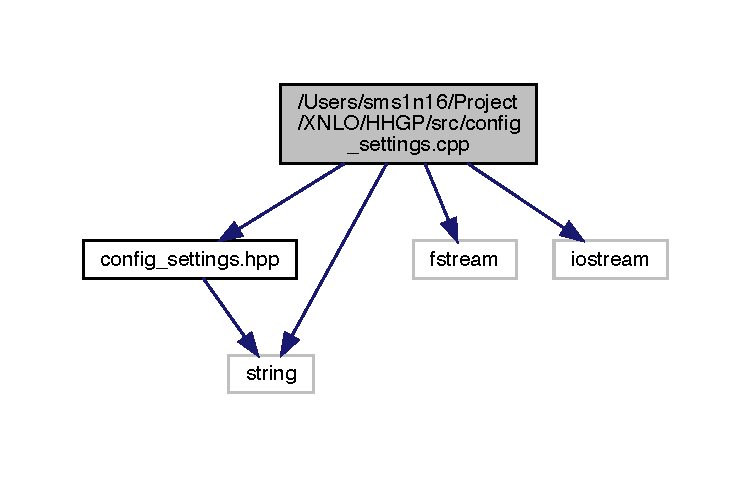
\includegraphics[width=350pt]{config__settings_8cpp__incl}
\end{center}
\end{figure}
\subsection*{Namespaces}
\begin{DoxyCompactItemize}
\item 
 \hyperlink{namespace_h_h}{HH}
\end{DoxyCompactItemize}

\hypertarget{config__settings_8hpp}{}\section{/\+Users/sms1n16/\+Project/\+X\+N\+L\+O/\+H\+H\+G\+P/src/config\+\_\+settings.hpp File Reference}
\label{config__settings_8hpp}\index{/\+Users/sms1n16/\+Project/\+X\+N\+L\+O/\+H\+H\+G\+P/src/config\+\_\+settings.\+hpp@{/\+Users/sms1n16/\+Project/\+X\+N\+L\+O/\+H\+H\+G\+P/src/config\+\_\+settings.\+hpp}}
{\ttfamily \#include $<$string$>$}\newline
Include dependency graph for config\+\_\+settings.\+hpp\+:\nopagebreak
\begin{figure}[H]
\begin{center}
\leavevmode
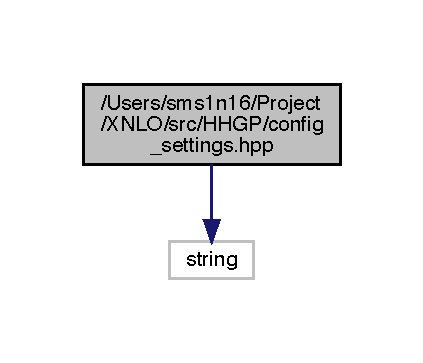
\includegraphics[width=203pt]{config__settings_8hpp__incl}
\end{center}
\end{figure}
This graph shows which files directly or indirectly include this file\+:\nopagebreak
\begin{figure}[H]
\begin{center}
\leavevmode
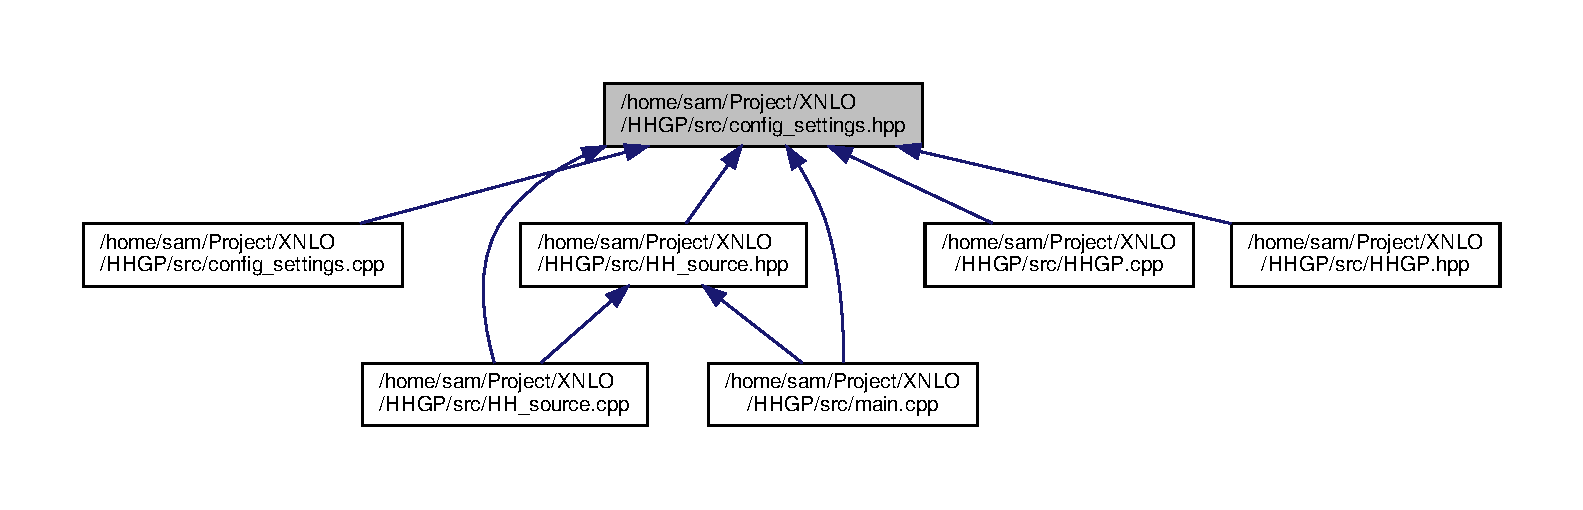
\includegraphics[width=350pt]{config__settings_8hpp__dep__incl}
\end{center}
\end{figure}
\subsection*{Classes}
\begin{DoxyCompactItemize}
\item 
class \hyperlink{class_config___settings}{Config\+\_\+\+Settings}
\end{DoxyCompactItemize}

\hypertarget{_d_h_t_8cpp}{}\section{/\+Users/sms1n16/\+Project/\+X\+N\+L\+O/src/\+D\+H\+T/\+D\+HT.cpp File Reference}
\label{_d_h_t_8cpp}\index{/Users/sms1n16/Project/XNLO/src/DHT/DHT.cpp@{/Users/sms1n16/Project/XNLO/src/DHT/DHT.cpp}}
{\ttfamily \#include \char`\"{}D\+H\+T.\+hpp\char`\"{}}\newline
{\ttfamily \#include \char`\"{}../../\+Eigen/\+Dense\char`\"{}}\newline
{\ttfamily \#include \char`\"{}../maths/maths\+\_\+textbook.\+hpp\char`\"{}}\newline

\hypertarget{_d_h_t_8hpp}{}\section{/home/sam/\+Project/\+X\+N\+L\+O/src/\+D\+H\+T/\+D\+HT.hpp File Reference}
\label{_d_h_t_8hpp}\index{/home/sam/Project/XNLO/src/DHT/DHT.hpp@{/home/sam/Project/XNLO/src/DHT/DHT.hpp}}
{\ttfamily \#include \char`\"{}../../\+Eigen/\+Dense\char`\"{}}\newline
{\ttfamily \#include \char`\"{}../maths/maths\+\_\+textbook.\+hpp\char`\"{}}\newline
Include dependency graph for D\+H\+T.\+hpp\+:
\nopagebreak
\begin{figure}[H]
\begin{center}
\leavevmode
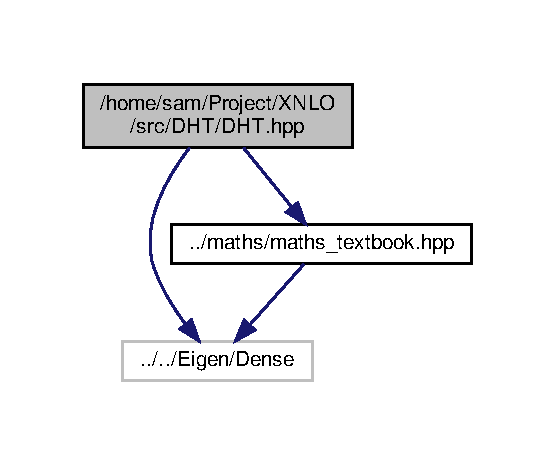
\includegraphics[width=267pt]{_d_h_t_8hpp__incl}
\end{center}
\end{figure}
This graph shows which files directly or indirectly include this file\+:
\nopagebreak
\begin{figure}[H]
\begin{center}
\leavevmode
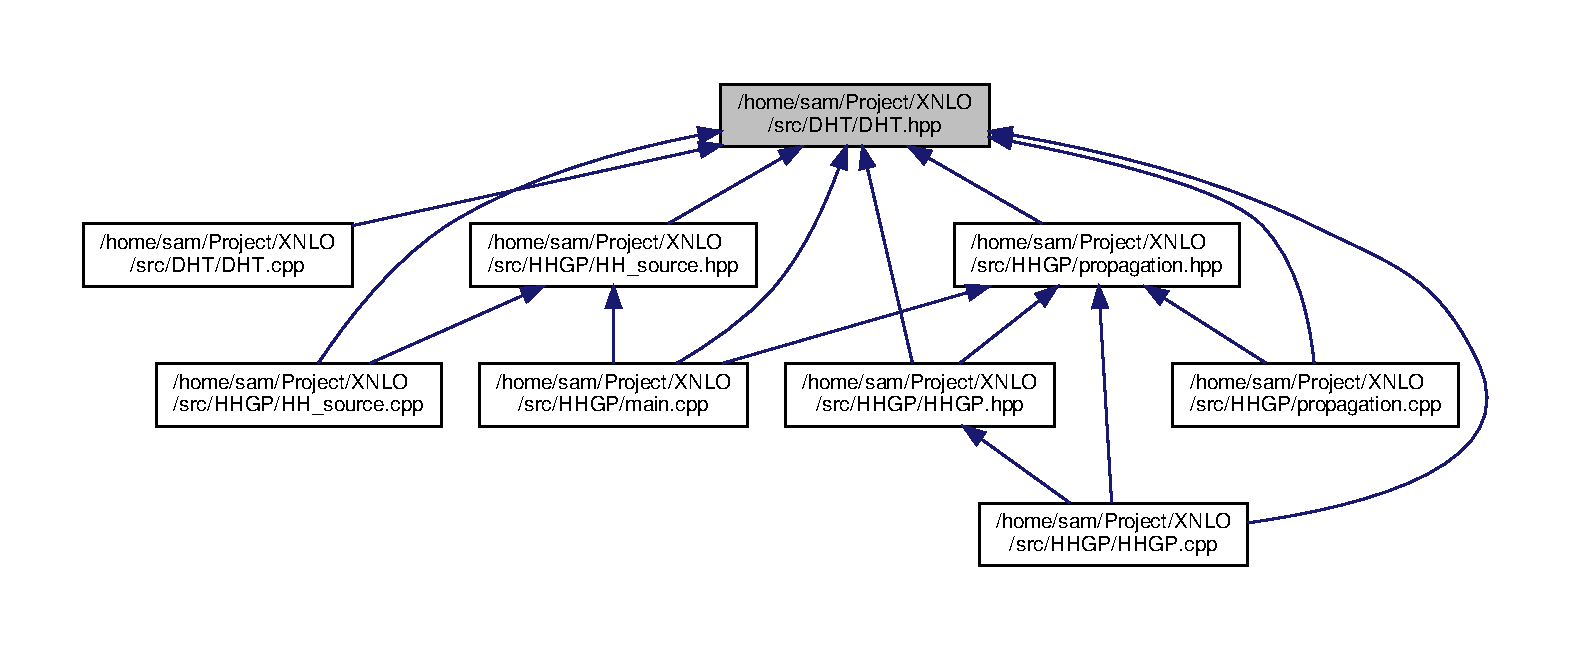
\includegraphics[width=350pt]{_d_h_t_8hpp__dep__incl}
\end{center}
\end{figure}
\subsection*{Classes}
\begin{DoxyCompactItemize}
\item 
class \mbox{\hyperlink{class_d_h_t}{D\+HT}}
\end{DoxyCompactItemize}

\hypertarget{grid__rkr_8cpp}{}\section{/home/sam/\+Project/\+X\+N\+L\+O/\+H\+H\+G\+P/src/grid\+\_\+rkr.cpp File Reference}
\label{grid__rkr_8cpp}\index{/home/sam/\+Project/\+X\+N\+L\+O/\+H\+H\+G\+P/src/grid\+\_\+rkr.\+cpp@{/home/sam/\+Project/\+X\+N\+L\+O/\+H\+H\+G\+P/src/grid\+\_\+rkr.\+cpp}}
{\ttfamily \#include \char`\"{}grid\+\_\+rkr.\+hpp\char`\"{}}\newline
{\ttfamily \#include \char`\"{}maths\+\_\+textbook.\+hpp\char`\"{}}\newline
{\ttfamily \#include \char`\"{}Eigen/\+Dense\char`\"{}}\newline
Include dependency graph for grid\+\_\+rkr.\+cpp\+:\nopagebreak
\begin{figure}[H]
\begin{center}
\leavevmode
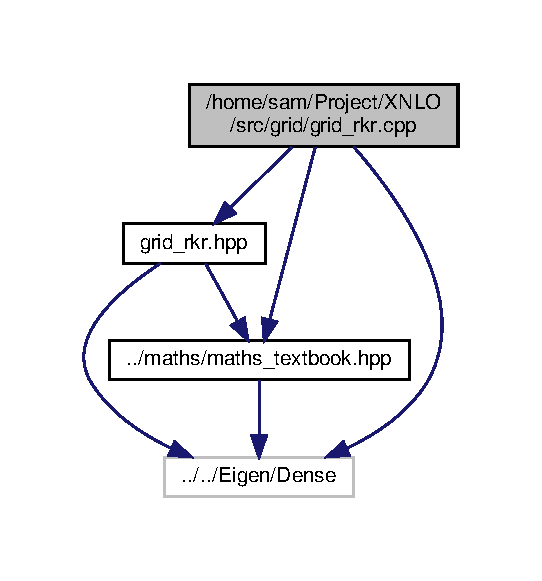
\includegraphics[width=251pt]{grid__rkr_8cpp__incl}
\end{center}
\end{figure}
\subsection*{Namespaces}
\begin{DoxyCompactItemize}
\item 
 \hyperlink{namespace_h_h_g_p}{H\+H\+GP}
\end{DoxyCompactItemize}

\hypertarget{grid__rkr_8hpp}{}\section{/home/sam/\+Project/\+X\+N\+L\+O/src/grid/grid\+\_\+rkr.hpp File Reference}
\label{grid__rkr_8hpp}\index{/home/sam/\+Project/\+X\+N\+L\+O/src/grid/grid\+\_\+rkr.\+hpp@{/home/sam/\+Project/\+X\+N\+L\+O/src/grid/grid\+\_\+rkr.\+hpp}}
{\ttfamily \#include \char`\"{}../../\+Eigen/\+Dense\char`\"{}}\newline
{\ttfamily \#include \char`\"{}../maths/maths\+\_\+textbook.\+hpp\char`\"{}}\newline
Include dependency graph for grid\+\_\+rkr.\+hpp\+:\nopagebreak
\begin{figure}[H]
\begin{center}
\leavevmode
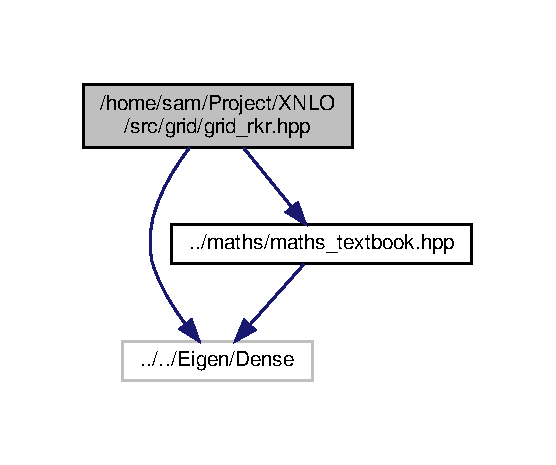
\includegraphics[width=267pt]{grid__rkr_8hpp__incl}
\end{center}
\end{figure}
This graph shows which files directly or indirectly include this file\+:\nopagebreak
\begin{figure}[H]
\begin{center}
\leavevmode
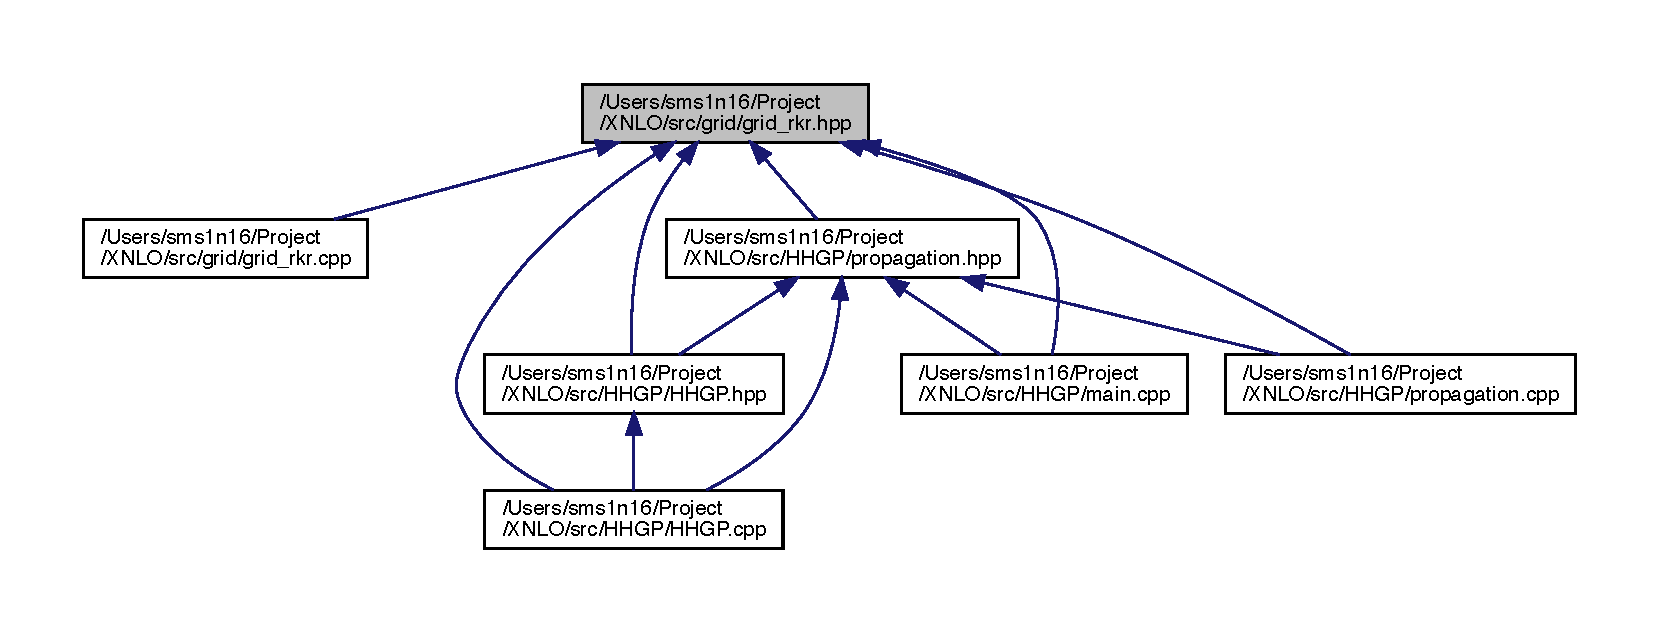
\includegraphics[width=350pt]{grid__rkr_8hpp__dep__incl}
\end{center}
\end{figure}
\subsection*{Classes}
\begin{DoxyCompactItemize}
\item 
class \hyperlink{classgrid__rkr}{grid\+\_\+rkr}
\end{DoxyCompactItemize}

\hypertarget{grid__tw_8cpp}{}\section{/\+Users/sms1n16/\+Project/\+X\+N\+L\+O/src/grid/grid\+\_\+tw.cpp File Reference}
\label{grid__tw_8cpp}\index{/Users/sms1n16/Project/XNLO/src/grid/grid\_tw.cpp@{/Users/sms1n16/Project/XNLO/src/grid/grid\_tw.cpp}}
{\ttfamily \#include \char`\"{}grid\+\_\+tw.\+hpp\char`\"{}}\newline
{\ttfamily \#include \char`\"{}../maths/maths\+\_\+textbook.\+hpp\char`\"{}}\newline
{\ttfamily \#include \char`\"{}../../\+Eigen/\+Dense\char`\"{}}\newline
{\ttfamily \#include $<$iostream$>$}\newline
Include dependency graph for grid\+\_\+tw.\+cpp\+:\nopagebreak
\begin{figure}[H]
\begin{center}
\leavevmode
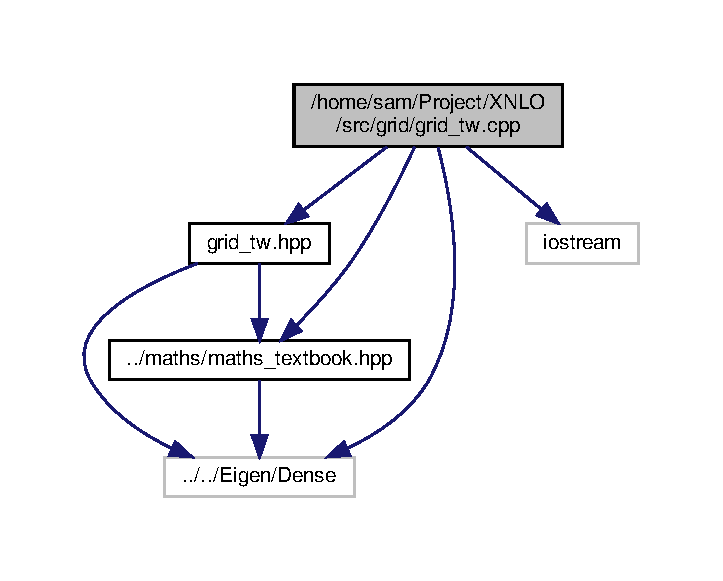
\includegraphics[width=347pt]{grid__tw_8cpp__incl}
\end{center}
\end{figure}
\subsection*{Namespaces}
\begin{DoxyCompactItemize}
\item 
 \mbox{\hyperlink{namespace_x_n_l_o}{X\+N\+LO}}
\end{DoxyCompactItemize}

\hypertarget{grid__tw_8hpp}{}\section{/\+Users/sms1n16/\+Project/\+X\+N\+L\+O/src/grid/grid\+\_\+tw.hpp File Reference}
\label{grid__tw_8hpp}\index{/Users/sms1n16/Project/XNLO/src/grid/grid\_tw.hpp@{/Users/sms1n16/Project/XNLO/src/grid/grid\_tw.hpp}}
{\ttfamily \#include \char`\"{}../../\+Eigen/\+Dense\char`\"{}}\newline
{\ttfamily \#include \char`\"{}../maths/maths\+\_\+textbook.\+hpp\char`\"{}}\newline
Include dependency graph for grid\+\_\+tw.\+hpp\+:\nopagebreak
\begin{figure}[H]
\begin{center}
\leavevmode
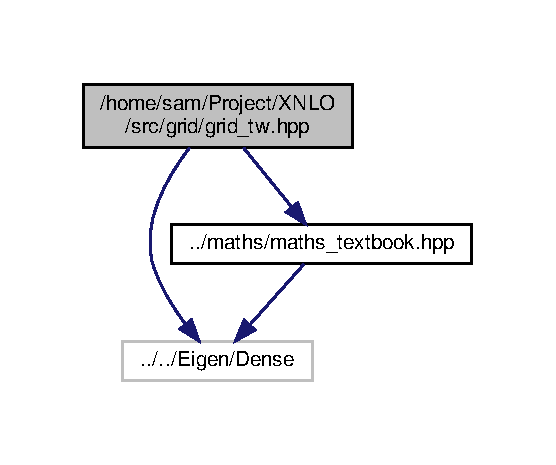
\includegraphics[width=270pt]{grid__tw_8hpp__incl}
\end{center}
\end{figure}
This graph shows which files directly or indirectly include this file\+:\nopagebreak
\begin{figure}[H]
\begin{center}
\leavevmode
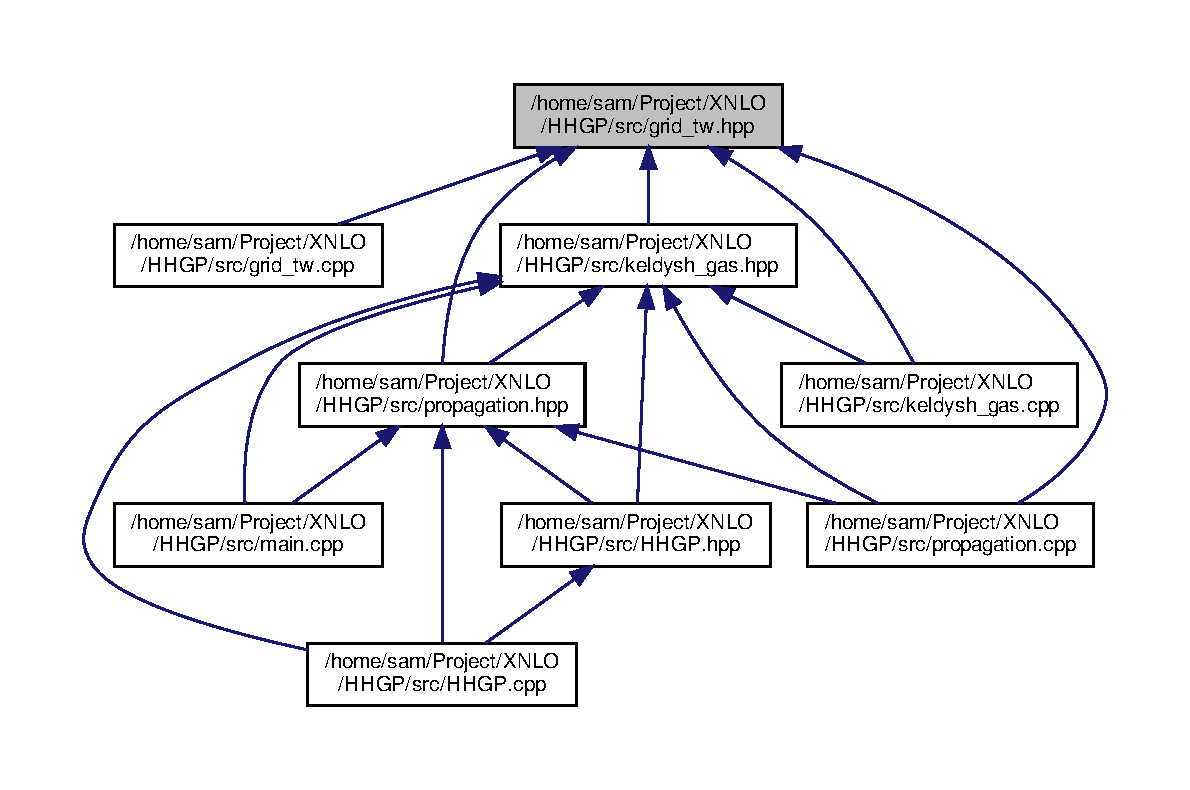
\includegraphics[width=350pt]{grid__tw_8hpp__dep__incl}
\end{center}
\end{figure}
\subsection*{Classes}
\begin{DoxyCompactItemize}
\item 
class \mbox{\hyperlink{classgrid__tw}{grid\+\_\+tw}}
\item 
class \mbox{\hyperlink{class_x_n_l_o_1_1grid__tw}{X\+N\+L\+O\+::grid\+\_\+tw}}
\end{DoxyCompactItemize}
\subsection*{Namespaces}
\begin{DoxyCompactItemize}
\item 
 \mbox{\hyperlink{namespace_x_n_l_o}{X\+N\+LO}}
\end{DoxyCompactItemize}

\hypertarget{_h_h__source_8cpp}{}\section{/home/sam/\+Project/\+X\+N\+L\+O/\+H\+H\+G\+P/src/\+H\+H\+\_\+source.cpp File Reference}
\label{_h_h__source_8cpp}\index{/home/sam/\+Project/\+X\+N\+L\+O/\+H\+H\+G\+P/src/\+H\+H\+\_\+source.\+cpp@{/home/sam/\+Project/\+X\+N\+L\+O/\+H\+H\+G\+P/src/\+H\+H\+\_\+source.\+cpp}}
{\ttfamily \#include $<$iostream$>$}\newline
{\ttfamily \#include $<$string$>$}\newline
{\ttfamily \#include \char`\"{}Eigen/\+Dense\char`\"{}}\newline
{\ttfamily \#include \char`\"{}H\+H\+\_\+source.\+hpp\char`\"{}}\newline
{\ttfamily \#include \char`\"{}../../src/\+I\+O.\+hpp\char`\"{}}\newline
{\ttfamily \#include \char`\"{}config\+\_\+settings.\+hpp\char`\"{}}\newline
{\ttfamily \#include \char`\"{}../../src/maths\+\_\+textbook.\+hpp\char`\"{}}\newline
{\ttfamily \#include \char`\"{}../../src/\+D\+H\+T.\+hpp\char`\"{}}\newline

\hypertarget{_h_h__source_8hpp}{}\section{/home/sam/\+Project/\+X\+N\+L\+O/src/\+H\+H\+G\+P/\+H\+H\+\_\+source.hpp File Reference}
\label{_h_h__source_8hpp}\index{/home/sam/Project/XNLO/src/HHGP/HH\_source.hpp@{/home/sam/Project/XNLO/src/HHGP/HH\_source.hpp}}
{\ttfamily \#include $<$iostream$>$}\newline
{\ttfamily \#include $<$string$>$}\newline
{\ttfamily \#include \char`\"{}../../\+Eigen/\+Dense\char`\"{}}\newline
{\ttfamily \#include \char`\"{}../\+I\+O/\+I\+O.\+hpp\char`\"{}}\newline
{\ttfamily \#include \char`\"{}config\+\_\+settings.\+hpp\char`\"{}}\newline
{\ttfamily \#include \char`\"{}../maths/maths\+\_\+textbook.\+hpp\char`\"{}}\newline
{\ttfamily \#include \char`\"{}../\+D\+H\+T/\+D\+H\+T.\+hpp\char`\"{}}\newline
Include dependency graph for H\+H\+\_\+source.\+hpp\+:
\nopagebreak
\begin{figure}[H]
\begin{center}
\leavevmode
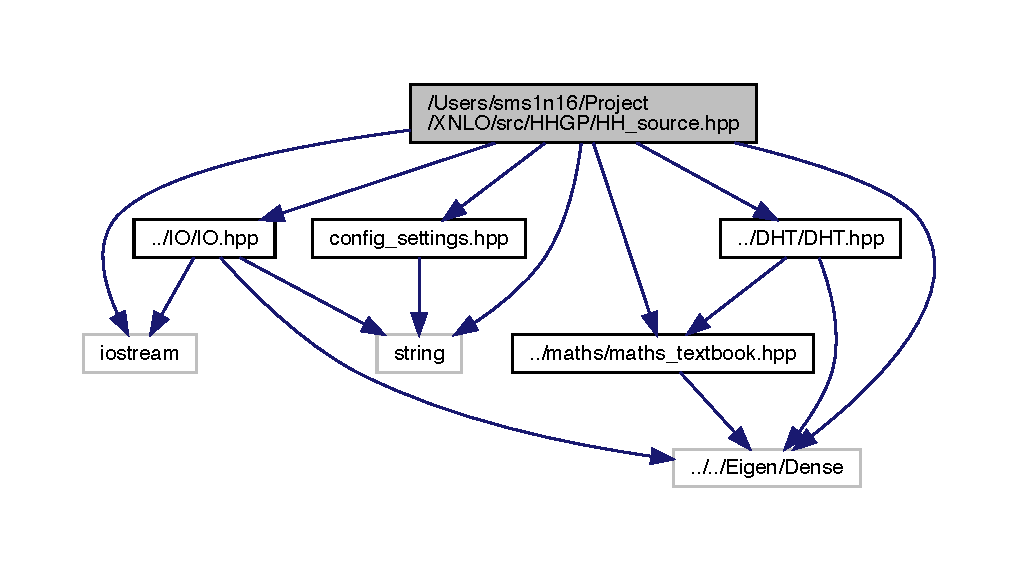
\includegraphics[width=350pt]{_h_h__source_8hpp__incl}
\end{center}
\end{figure}
This graph shows which files directly or indirectly include this file\+:
\nopagebreak
\begin{figure}[H]
\begin{center}
\leavevmode
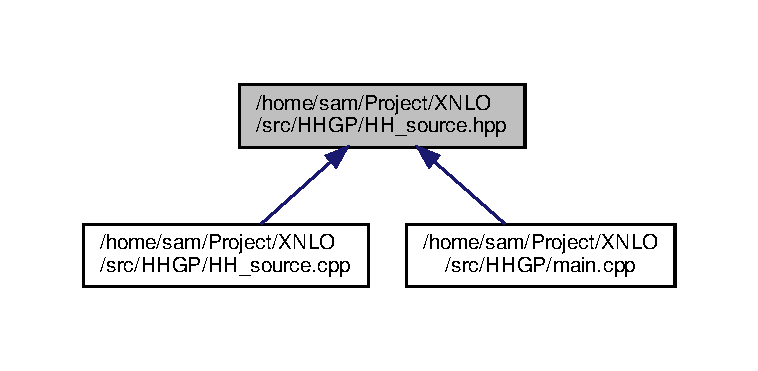
\includegraphics[width=350pt]{_h_h__source_8hpp__dep__incl}
\end{center}
\end{figure}
\subsection*{Classes}
\begin{DoxyCompactItemize}
\item 
class \mbox{\hyperlink{class_h_h__source}{H\+H\+\_\+source}}
\end{DoxyCompactItemize}

\hypertarget{_h_h_g_p_8cpp}{}\section{/home/sam/\+Project/\+X\+N\+L\+O/\+H\+H\+G\+P/src/\+H\+H\+GP.cpp File Reference}
\label{_h_h_g_p_8cpp}\index{/home/sam/\+Project/\+X\+N\+L\+O/\+H\+H\+G\+P/src/\+H\+H\+G\+P.\+cpp@{/home/sam/\+Project/\+X\+N\+L\+O/\+H\+H\+G\+P/src/\+H\+H\+G\+P.\+cpp}}
{\ttfamily \#include $<$iostream$>$}\newline
{\ttfamily \#include $<$string$>$}\newline
{\ttfamily \#include \char`\"{}../../\+Eigen/\+Dense\char`\"{}}\newline
{\ttfamily \#include \char`\"{}H\+H\+G\+P.\+hpp\char`\"{}}\newline
{\ttfamily \#include \char`\"{}config\+\_\+settings.\+hpp\char`\"{}}\newline
{\ttfamily \#include \char`\"{}../../src/maths\+\_\+textbook.\+hpp\char`\"{}}\newline
{\ttfamily \#include \char`\"{}../../src/keldysh\+\_\+gas.\+hpp\char`\"{}}\newline
{\ttfamily \#include \char`\"{}../../src/\+D\+H\+T.\+hpp\char`\"{}}\newline
{\ttfamily \#include \char`\"{}../../src/grid\+\_\+rkr.\+hpp\char`\"{}}\newline
{\ttfamily \#include \char`\"{}propagation.\+hpp\char`\"{}}\newline
{\ttfamily \#include \char`\"{}../../src/\+I\+O.\+hpp\char`\"{}}\newline
Include dependency graph for H\+H\+G\+P.\+cpp\+:
\nopagebreak
\begin{figure}[H]
\begin{center}
\leavevmode
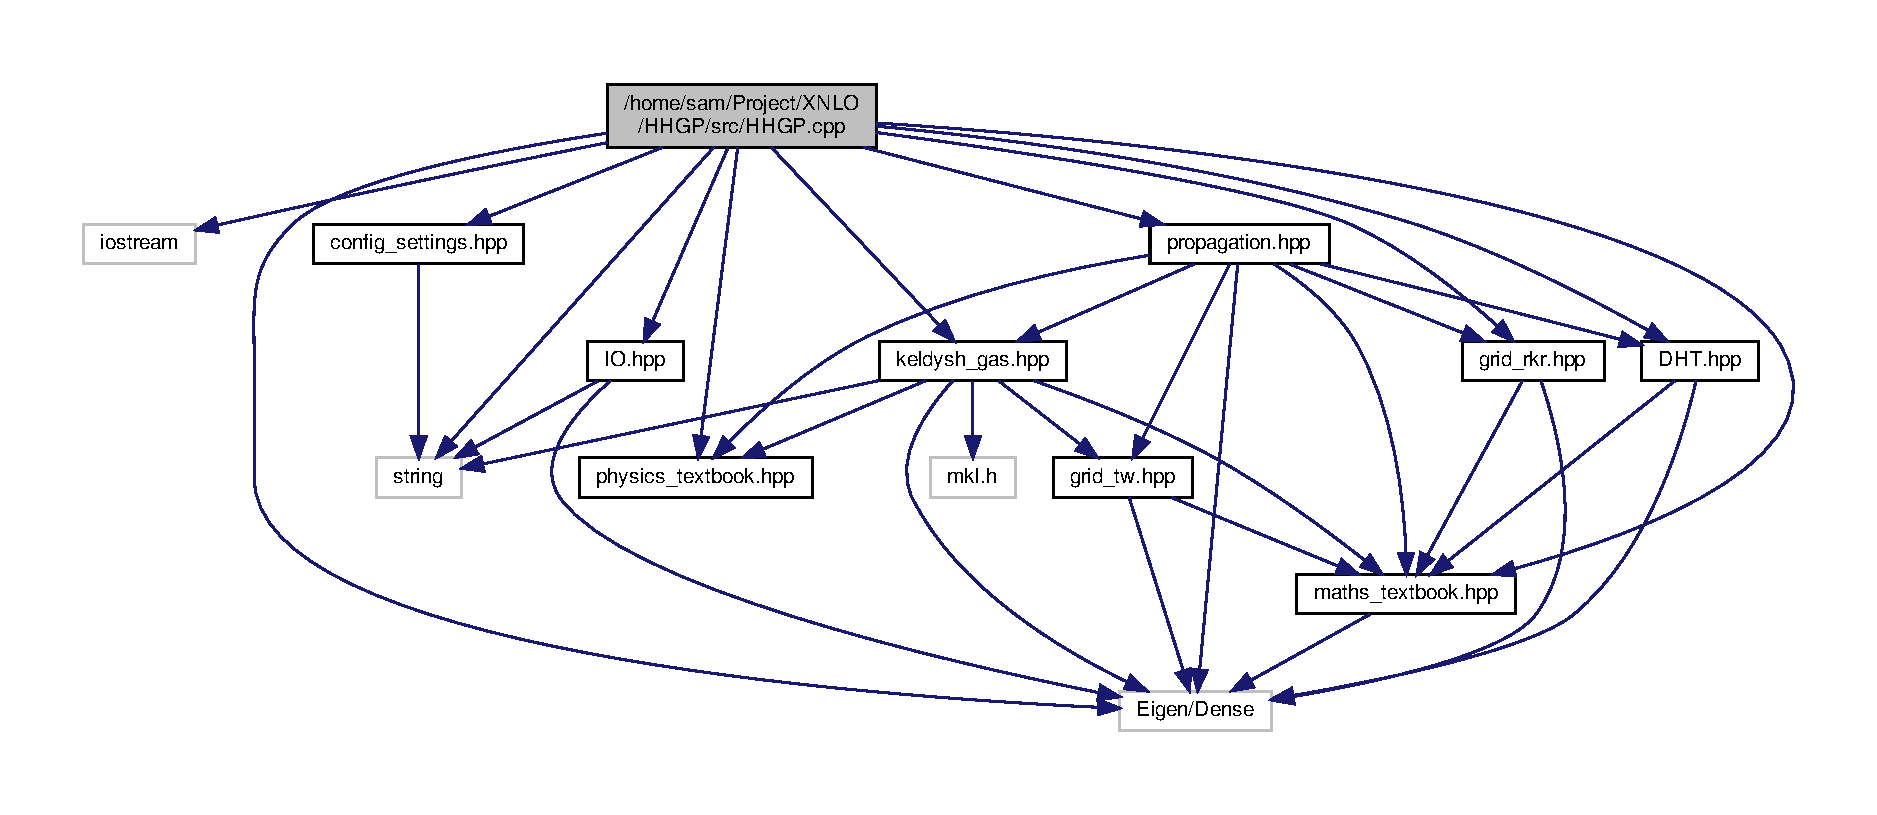
\includegraphics[width=350pt]{_h_h_g_p_8cpp__incl}
\end{center}
\end{figure}

\hypertarget{_h_h_g_p_8hpp}{}\section{/home/sam/\+Project/\+X\+N\+L\+O/src/\+H\+H\+G\+P/\+H\+H\+GP.hpp File Reference}
\label{_h_h_g_p_8hpp}\index{/home/sam/\+Project/\+X\+N\+L\+O/src/\+H\+H\+G\+P/\+H\+H\+G\+P.\+hpp@{/home/sam/\+Project/\+X\+N\+L\+O/src/\+H\+H\+G\+P/\+H\+H\+G\+P.\+hpp}}
{\ttfamily \#include \char`\"{}../../\+Eigen/\+Dense\char`\"{}}\newline
{\ttfamily \#include \char`\"{}config\+\_\+settings.\+hpp\char`\"{}}\newline
{\ttfamily \#include \char`\"{}../maths/maths\+\_\+textbook.\+hpp\char`\"{}}\newline
{\ttfamily \#include \char`\"{}../physics/physics\+\_\+textbook.\+hpp\char`\"{}}\newline
{\ttfamily \#include \char`\"{}../gas/keldysh\+\_\+gas.\+hpp\char`\"{}}\newline
{\ttfamily \#include \char`\"{}../\+D\+H\+T/\+D\+H\+T.\+hpp\char`\"{}}\newline
{\ttfamily \#include \char`\"{}../grid/grid\+\_\+rkr.\+hpp\char`\"{}}\newline
{\ttfamily \#include \char`\"{}propagation.\+hpp\char`\"{}}\newline
{\ttfamily \#include \char`\"{}../\+I\+O/\+I\+O.\+hpp\char`\"{}}\newline
Include dependency graph for H\+H\+G\+P.\+hpp\+:\nopagebreak
\begin{figure}[H]
\begin{center}
\leavevmode
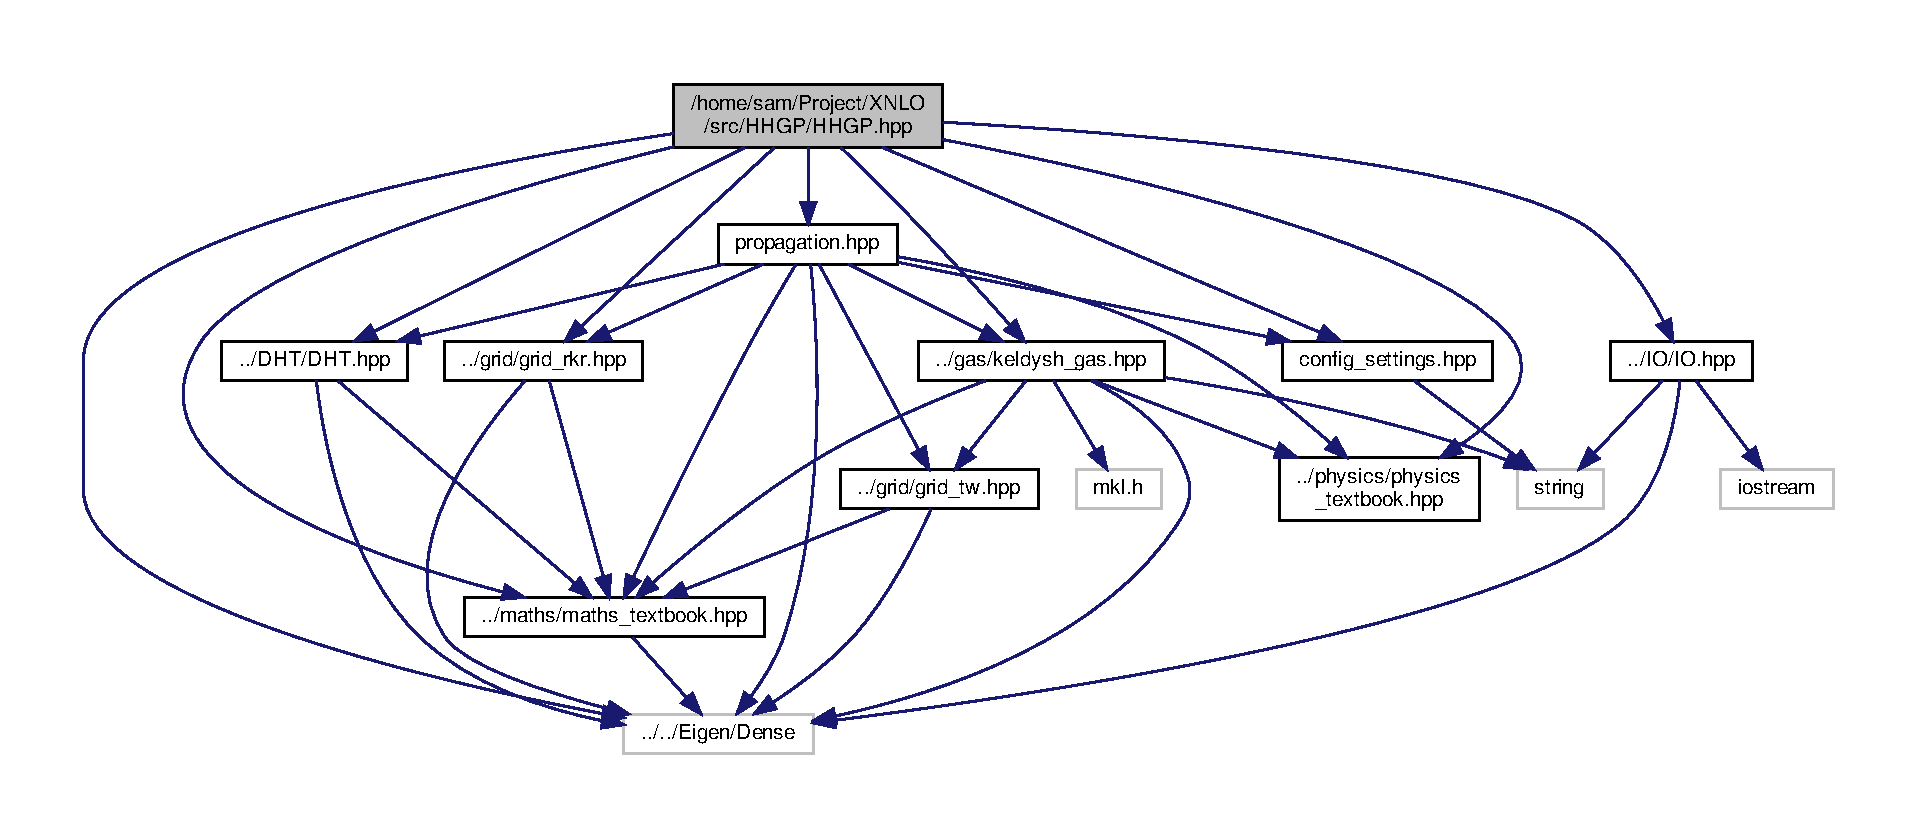
\includegraphics[width=350pt]{_h_h_g_p_8hpp__incl}
\end{center}
\end{figure}
This graph shows which files directly or indirectly include this file\+:\nopagebreak
\begin{figure}[H]
\begin{center}
\leavevmode
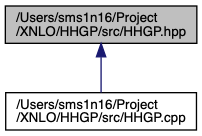
\includegraphics[width=209pt]{_h_h_g_p_8hpp__dep__incl}
\end{center}
\end{figure}
\subsection*{Classes}
\begin{DoxyCompactItemize}
\item 
class \hyperlink{class_h_h_g_p}{H\+H\+GP}
\end{DoxyCompactItemize}

\hypertarget{_i_o_8cpp}{}\section{/home/sam/\+Project/\+X\+N\+L\+O/\+H\+H\+G\+P/src/\+IO.cpp File Reference}
\label{_i_o_8cpp}\index{/home/sam/\+Project/\+X\+N\+L\+O/\+H\+H\+G\+P/src/\+I\+O.\+cpp@{/home/sam/\+Project/\+X\+N\+L\+O/\+H\+H\+G\+P/src/\+I\+O.\+cpp}}
{\ttfamily \#include \char`\"{}I\+O.\+hpp\char`\"{}}\newline
{\ttfamily \#include \char`\"{}Eigen/\+Dense\char`\"{}}\newline
{\ttfamily \#include $<$fstream$>$}\newline
{\ttfamily \#include $<$iostream$>$}\newline
{\ttfamily \#include $<$string$>$}\newline
Include dependency graph for I\+O.\+cpp\+:\nopagebreak
\begin{figure}[H]
\begin{center}
\leavevmode
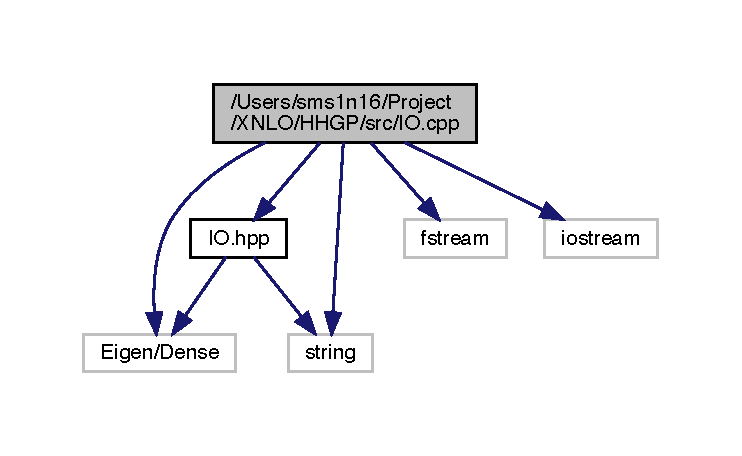
\includegraphics[width=350pt]{_i_o_8cpp__incl}
\end{center}
\end{figure}

\hypertarget{_i_o_8hpp}{}\section{/home/sam/\+Project/\+X\+N\+L\+O/\+H\+H\+G\+P/src/\+IO.hpp File Reference}
\label{_i_o_8hpp}\index{/home/sam/\+Project/\+X\+N\+L\+O/\+H\+H\+G\+P/src/\+I\+O.\+hpp@{/home/sam/\+Project/\+X\+N\+L\+O/\+H\+H\+G\+P/src/\+I\+O.\+hpp}}
{\ttfamily \#include \char`\"{}Eigen/\+Dense\char`\"{}}\newline
{\ttfamily \#include $<$string$>$}\newline
Include dependency graph for I\+O.\+hpp\+:\nopagebreak
\begin{figure}[H]
\begin{center}
\leavevmode
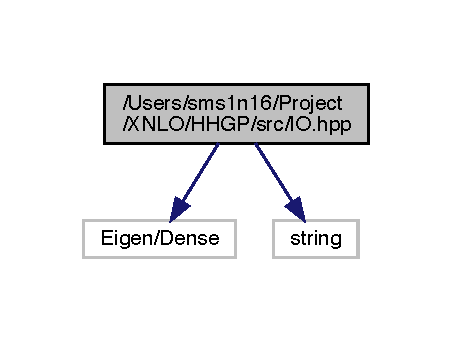
\includegraphics[width=217pt]{_i_o_8hpp__incl}
\end{center}
\end{figure}
This graph shows which files directly or indirectly include this file\+:
\nopagebreak
\begin{figure}[H]
\begin{center}
\leavevmode
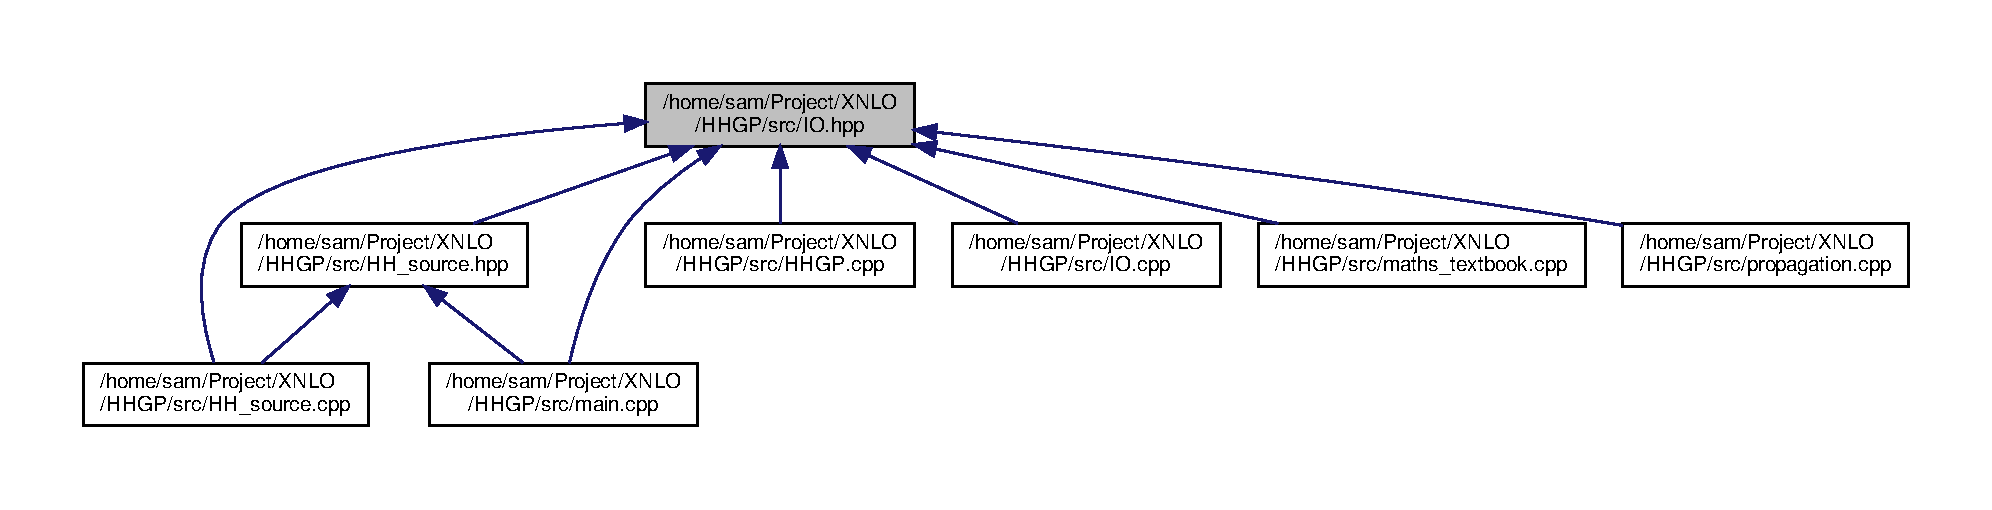
\includegraphics[width=350pt]{_i_o_8hpp__dep__incl}
\end{center}
\end{figure}
\subsection*{Classes}
\begin{DoxyCompactItemize}
\item 
class \hyperlink{class_i_o}{IO}
\end{DoxyCompactItemize}

\hypertarget{keldysh__gas_8cpp}{}\section{/\+Users/sms1n16/\+Project/\+X\+N\+L\+O/src/gas/keldysh\+\_\+gas.cpp File Reference}
\label{keldysh__gas_8cpp}\index{/\+Users/sms1n16/\+Project/\+X\+N\+L\+O/src/gas/keldysh\+\_\+gas.\+cpp@{/\+Users/sms1n16/\+Project/\+X\+N\+L\+O/src/gas/keldysh\+\_\+gas.\+cpp}}
{\ttfamily \#include \char`\"{}keldysh\+\_\+gas.\+hpp\char`\"{}}\newline
{\ttfamily \#include \char`\"{}../physics/physics\+\_\+textbook.\+hpp\char`\"{}}\newline
{\ttfamily \#include \char`\"{}../grid/grid\+\_\+tw.\+hpp\char`\"{}}\newline
{\ttfamily \#include $<$mkl.\+h$>$}\newline
{\ttfamily \#include \char`\"{}../../\+Eigen/\+Dense\char`\"{}}\newline
{\ttfamily \#include \char`\"{}../maths/maths\+\_\+textbook.\+hpp\char`\"{}}\newline
{\ttfamily \#include $<$cmath$>$}\newline
{\ttfamily \#include $<$iostream$>$}\newline
Include dependency graph for keldysh\+\_\+gas.\+cpp\+:\nopagebreak
\begin{figure}[H]
\begin{center}
\leavevmode
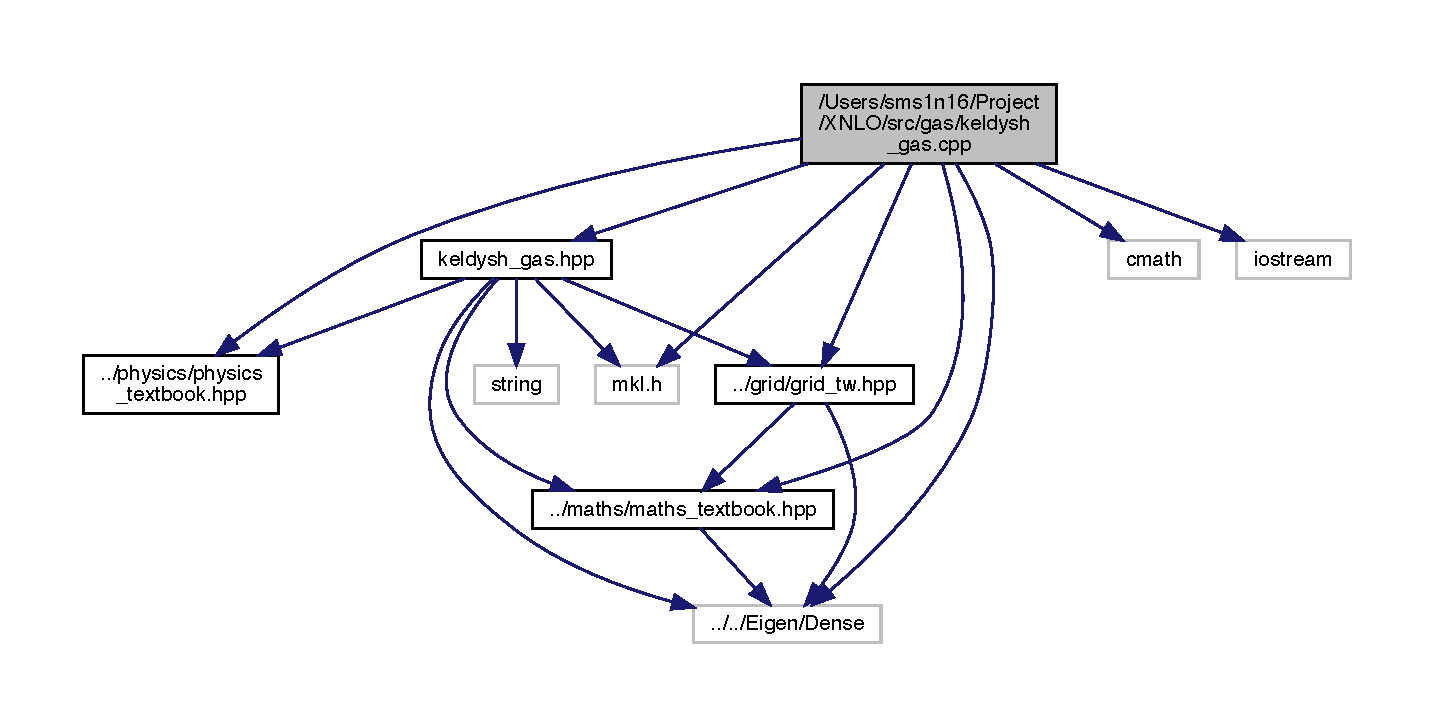
\includegraphics[width=350pt]{keldysh__gas_8cpp__incl}
\end{center}
\end{figure}

\hypertarget{keldysh__gas_8hpp}{}\section{/\+Users/sms1n16/\+Project/\+X\+N\+L\+O/src/gas/keldysh\+\_\+gas.hpp File Reference}
\label{keldysh__gas_8hpp}\index{/Users/sms1n16/Project/XNLO/src/gas/keldysh\_gas.hpp@{/Users/sms1n16/Project/XNLO/src/gas/keldysh\_gas.hpp}}
{\ttfamily \#include \char`\"{}../physics/physics\+\_\+textbook.\+hpp\char`\"{}}\newline
{\ttfamily \#include \char`\"{}../maths/maths\+\_\+textbook.\+hpp\char`\"{}}\newline
{\ttfamily \#include \char`\"{}../grid/grid\+\_\+tw.\+hpp\char`\"{}}\newline
{\ttfamily \#include $<$mkl.\+h$>$}\newline
{\ttfamily \#include \char`\"{}../../\+Eigen/\+Dense\char`\"{}}\newline
{\ttfamily \#include $<$string$>$}\newline
Include dependency graph for keldysh\+\_\+gas.\+hpp\+:\nopagebreak
\begin{figure}[H]
\begin{center}
\leavevmode
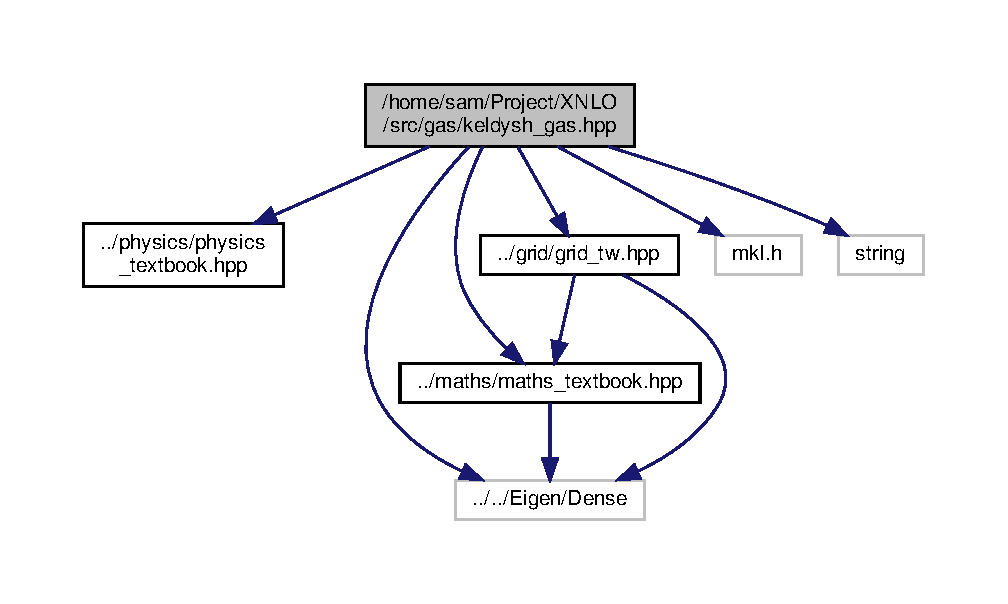
\includegraphics[width=350pt]{keldysh__gas_8hpp__incl}
\end{center}
\end{figure}
This graph shows which files directly or indirectly include this file\+:\nopagebreak
\begin{figure}[H]
\begin{center}
\leavevmode
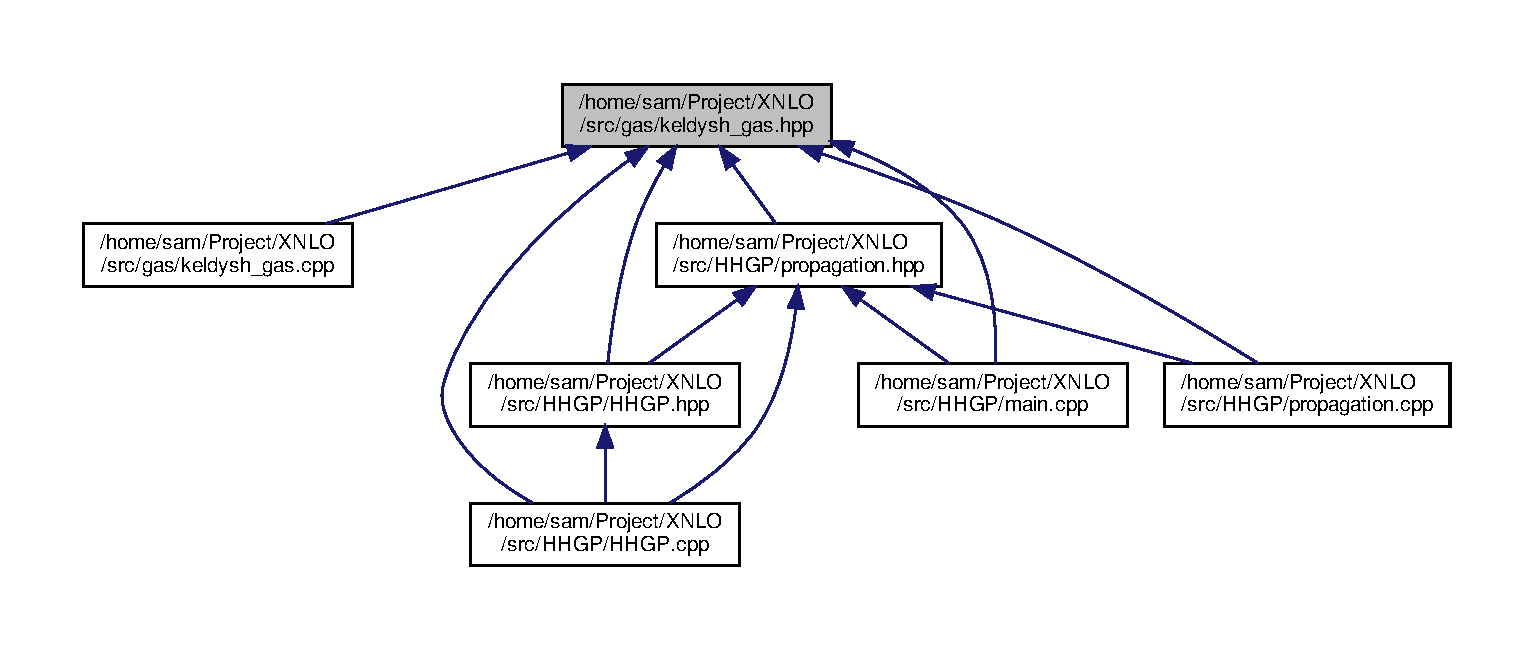
\includegraphics[width=350pt]{keldysh__gas_8hpp__dep__incl}
\end{center}
\end{figure}
\subsection*{Classes}
\begin{DoxyCompactItemize}
\item 
class \mbox{\hyperlink{classkeldysh__gas}{keldysh\+\_\+gas}}
\end{DoxyCompactItemize}

\hypertarget{main_8cpp}{}\section{/home/sam/\+Project/\+X\+N\+L\+O/src/\+H\+H\+G\+P/main.cpp File Reference}
\label{main_8cpp}\index{/home/sam/Project/XNLO/src/HHGP/main.cpp@{/home/sam/Project/XNLO/src/HHGP/main.cpp}}
{\ttfamily \#include $<$iostream$>$}\newline
{\ttfamily \#include $<$string$>$}\newline
{\ttfamily \#include \char`\"{}../../\+Eigen/\+Dense\char`\"{}}\newline
{\ttfamily \#include \char`\"{}config\+\_\+settings.\+hpp\char`\"{}}\newline
{\ttfamily \#include \char`\"{}../maths/maths\+\_\+textbook.\+hpp\char`\"{}}\newline
{\ttfamily \#include \char`\"{}../physics/physics\+\_\+textbook.\+hpp\char`\"{}}\newline
{\ttfamily \#include \char`\"{}H\+H\+\_\+source.\+hpp\char`\"{}}\newline
{\ttfamily \#include \char`\"{}../gas/keldysh\+\_\+gas.\+hpp\char`\"{}}\newline
{\ttfamily \#include \char`\"{}../\+D\+H\+T/\+D\+H\+T.\+hpp\char`\"{}}\newline
{\ttfamily \#include \char`\"{}../grid/grid\+\_\+rkr.\+hpp\char`\"{}}\newline
{\ttfamily \#include \char`\"{}propagation.\+hpp\char`\"{}}\newline
{\ttfamily \#include \char`\"{}../\+I\+O/\+I\+O.\+hpp\char`\"{}}\newline
Include dependency graph for main.\+cpp\+:\nopagebreak
\begin{figure}[H]
\begin{center}
\leavevmode
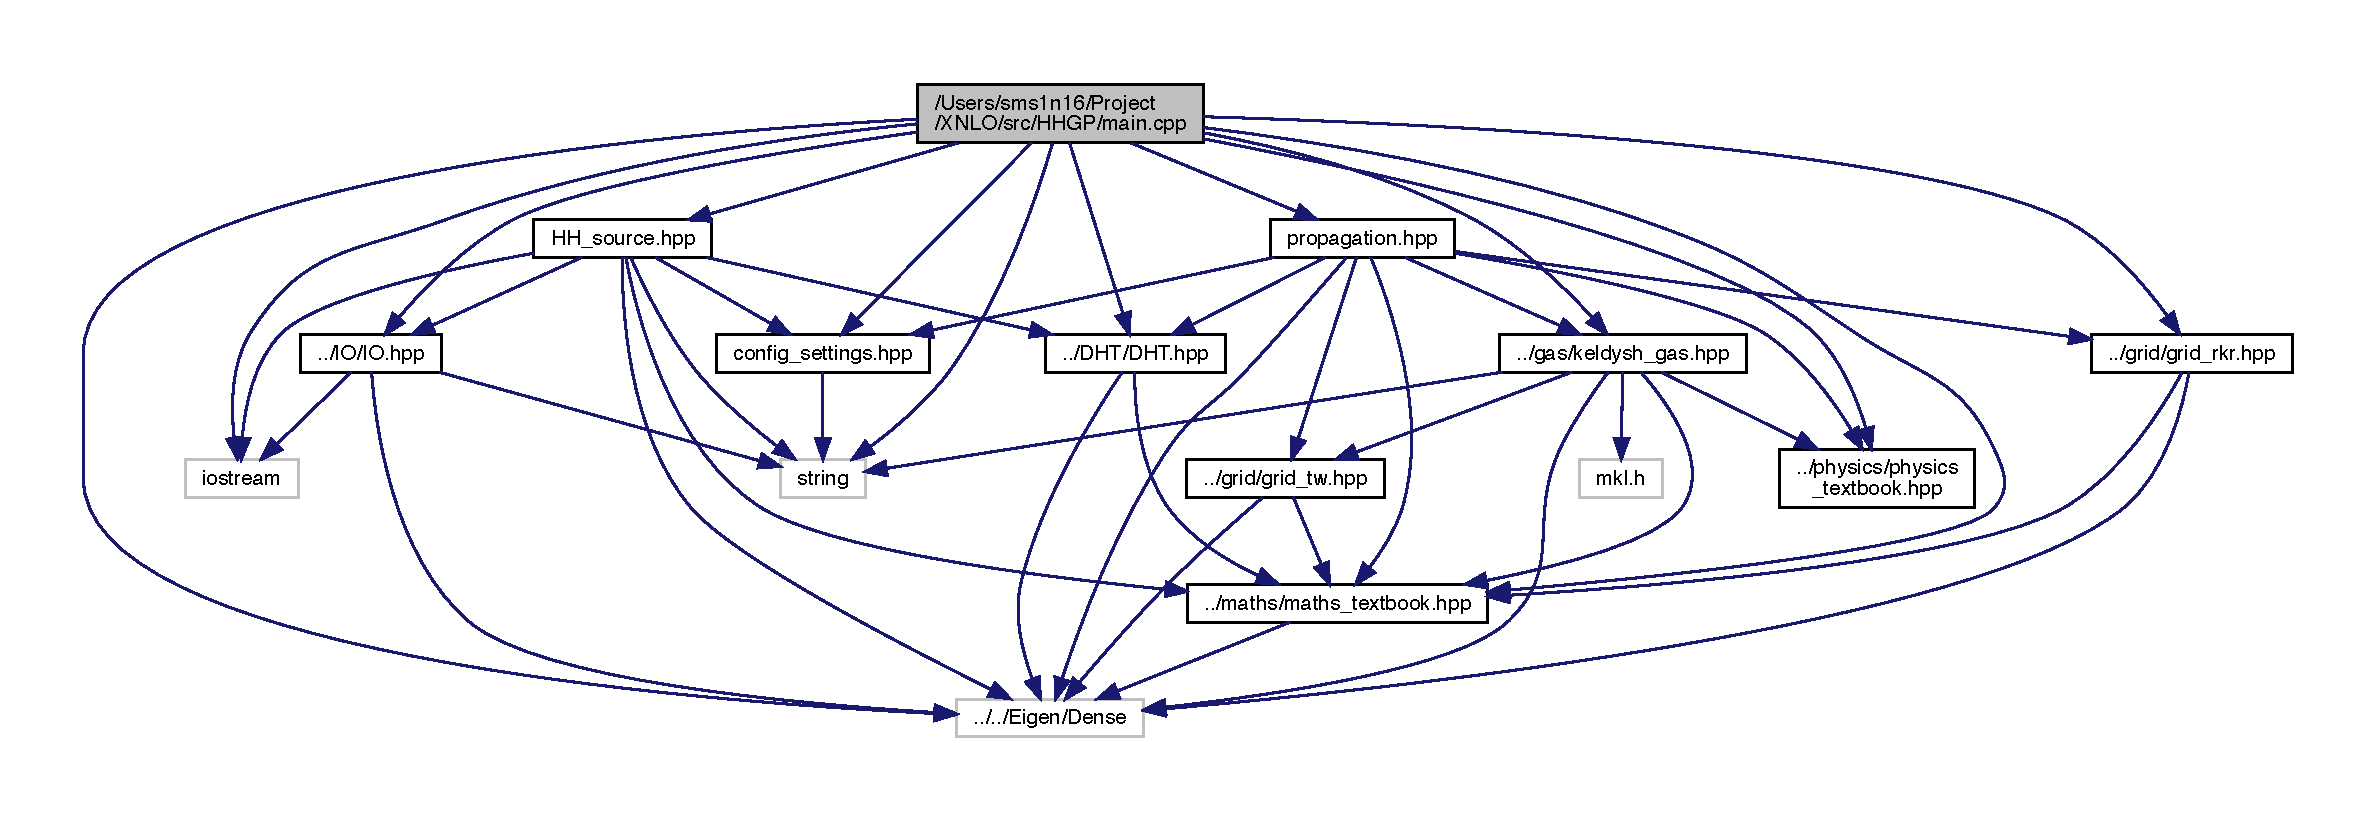
\includegraphics[width=350pt]{main_8cpp__incl}
\end{center}
\end{figure}
\subsection*{Functions}
\begin{DoxyCompactItemize}
\item 
int \mbox{\hyperlink{main_8cpp_a3c04138a5bfe5d72780bb7e82a18e627}{main}} (int argc, char $\ast$$\ast$argv)
\end{DoxyCompactItemize}


\subsection{Function Documentation}
\mbox{\Hypertarget{main_8cpp_a3c04138a5bfe5d72780bb7e82a18e627}\label{main_8cpp_a3c04138a5bfe5d72780bb7e82a18e627}} 
\index{main.cpp@{main.cpp}!main@{main}}
\index{main@{main}!main.cpp@{main.cpp}}
\subsubsection{\texorpdfstring{main()}{main()}}
{\footnotesize\ttfamily int main (\begin{DoxyParamCaption}\item[{int}]{argc,  }\item[{char $\ast$$\ast$}]{argv }\end{DoxyParamCaption})}

2.\+0; 
\hypertarget{maths__textbook_8cpp}{}\section{/home/sam/\+Project/\+X\+N\+L\+O/src/maths/maths\+\_\+textbook.cpp File Reference}
\label{maths__textbook_8cpp}\index{/home/sam/Project/XNLO/src/maths/maths\_textbook.cpp@{/home/sam/Project/XNLO/src/maths/maths\_textbook.cpp}}
{\ttfamily \#include \char`\"{}maths\+\_\+textbook.\+hpp\char`\"{}}\newline
{\ttfamily \#include \char`\"{}../\+I\+O/\+I\+O.\+hpp\char`\"{}}\newline
{\ttfamily \#include $<$cmath$>$}\newline
{\ttfamily \#include \char`\"{}../../\+Eigen/\+Dense\char`\"{}}\newline
{\ttfamily \#include $<$mkl.\+h$>$}\newline
{\ttfamily \#include $<$iostream$>$}\newline
Include dependency graph for maths\+\_\+textbook.\+cpp\+:
\nopagebreak
\begin{figure}[H]
\begin{center}
\leavevmode
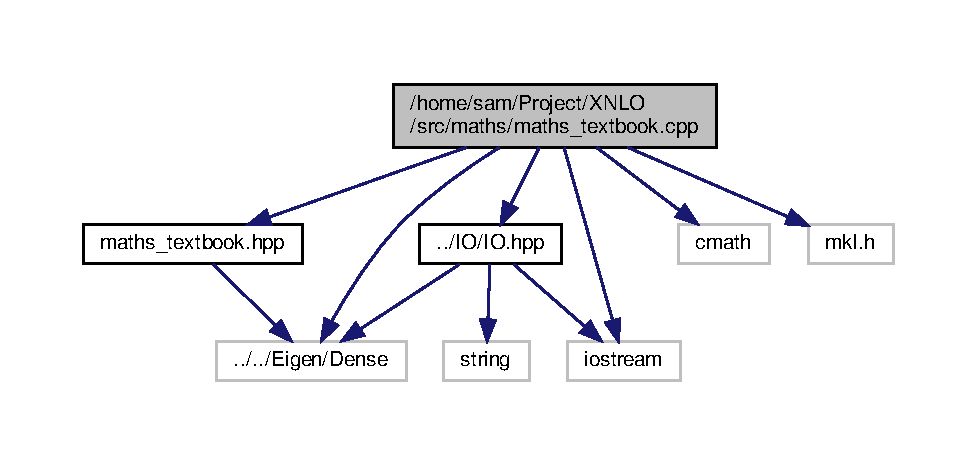
\includegraphics[width=350pt]{maths__textbook_8cpp__incl}
\end{center}
\end{figure}

\hypertarget{maths__textbook_8hpp}{}\section{/home/sam/\+Project/\+X\+N\+L\+O/\+H\+H\+G\+P/src/maths\+\_\+textbook.hpp File Reference}
\label{maths__textbook_8hpp}\index{/home/sam/\+Project/\+X\+N\+L\+O/\+H\+H\+G\+P/src/maths\+\_\+textbook.\+hpp@{/home/sam/\+Project/\+X\+N\+L\+O/\+H\+H\+G\+P/src/maths\+\_\+textbook.\+hpp}}
{\ttfamily \#include \char`\"{}Eigen/\+Dense\char`\"{}}\newline
Include dependency graph for maths\+\_\+textbook.\+hpp\+:\nopagebreak
\begin{figure}[H]
\begin{center}
\leavevmode
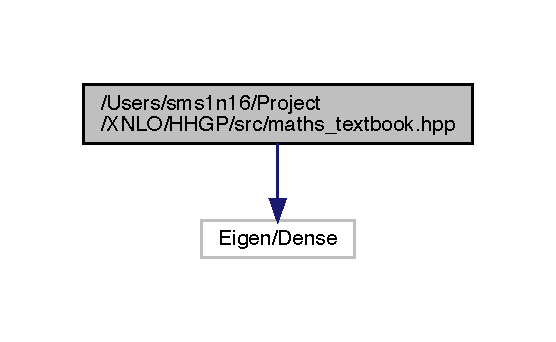
\includegraphics[width=267pt]{maths__textbook_8hpp__incl}
\end{center}
\end{figure}
This graph shows which files directly or indirectly include this file\+:\nopagebreak
\begin{figure}[H]
\begin{center}
\leavevmode
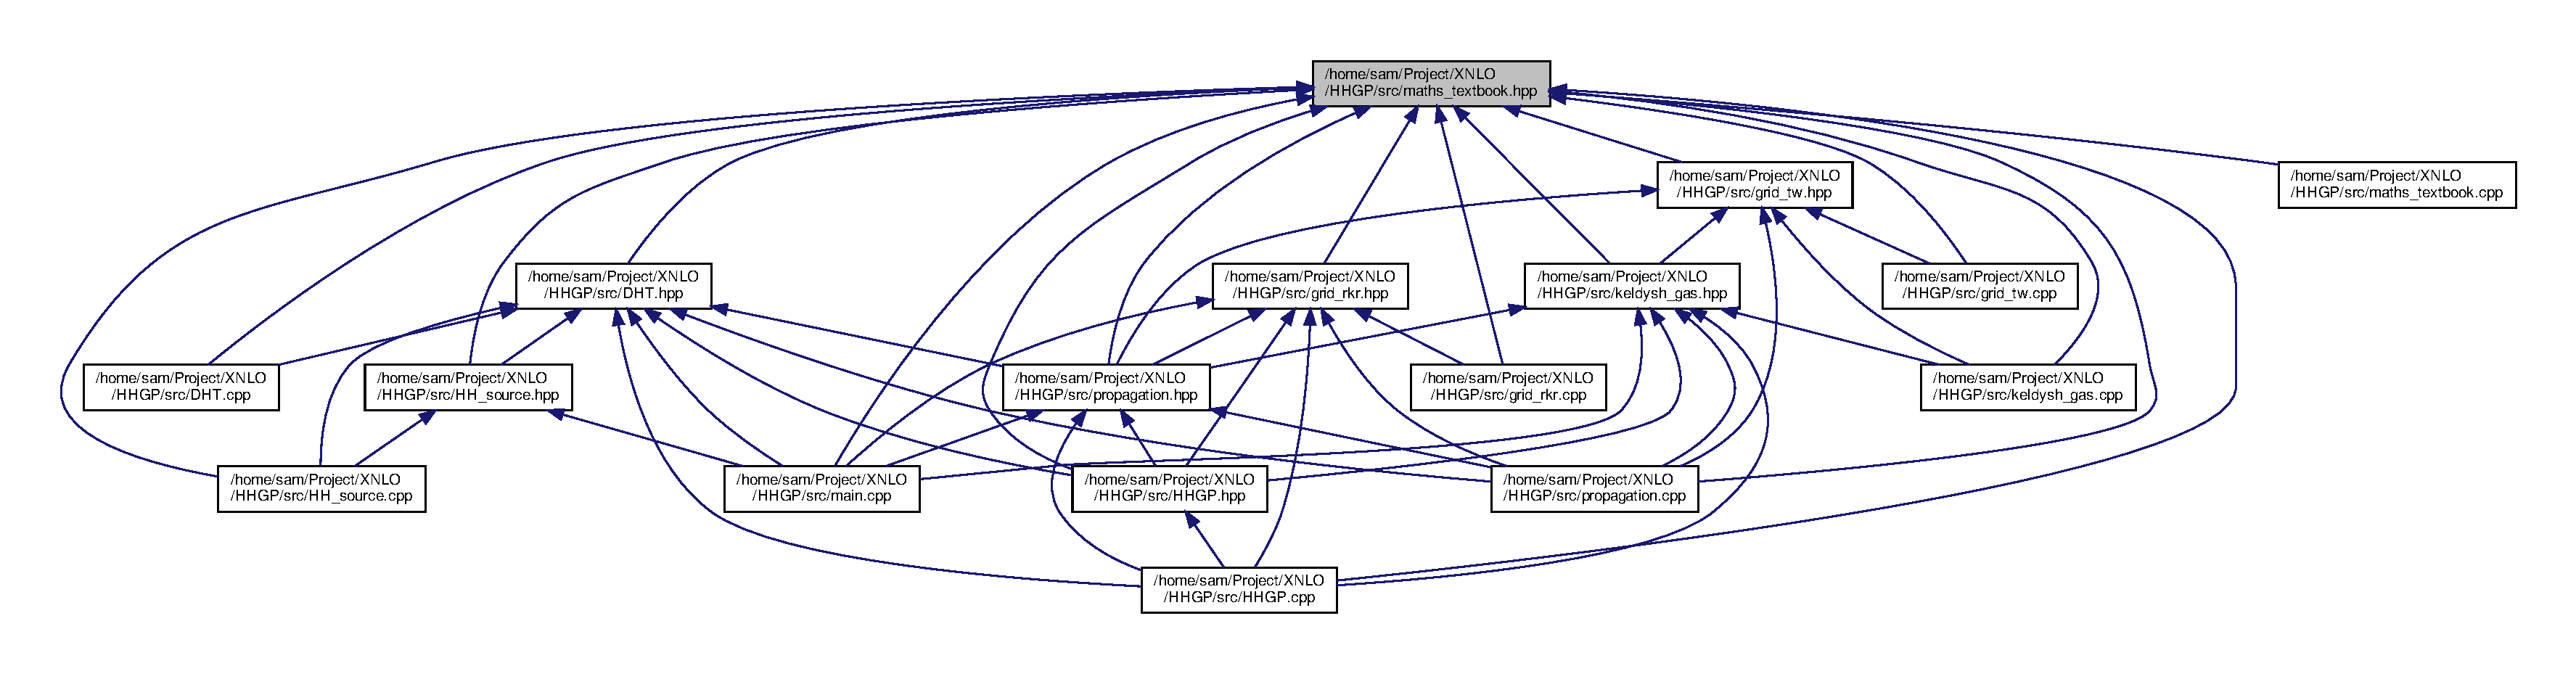
\includegraphics[width=350pt]{maths__textbook_8hpp__dep__incl}
\end{center}
\end{figure}
\subsection*{Classes}
\begin{DoxyCompactItemize}
\item 
class \hyperlink{class_h_h_g_p_1_1maths__textbook}{H\+H\+G\+P\+::maths\+\_\+textbook}
\end{DoxyCompactItemize}
\subsection*{Namespaces}
\begin{DoxyCompactItemize}
\item 
 \hyperlink{namespace_h_h_g_p}{H\+H\+GP}
\end{DoxyCompactItemize}

\hypertarget{physics__textbook_8cpp}{}\section{/home/sam/\+Project/\+X\+N\+L\+O/\+H\+H\+G\+P/src/physics\+\_\+textbook.cpp File Reference}
\label{physics__textbook_8cpp}\index{/home/sam/\+Project/\+X\+N\+L\+O/\+H\+H\+G\+P/src/physics\+\_\+textbook.\+cpp@{/home/sam/\+Project/\+X\+N\+L\+O/\+H\+H\+G\+P/src/physics\+\_\+textbook.\+cpp}}
{\ttfamily \#include \char`\"{}physics\+\_\+textbook.\+hpp\char`\"{}}\newline
Include dependency graph for physics\+\_\+textbook.\+cpp\+:\nopagebreak
\begin{figure}[H]
\begin{center}
\leavevmode
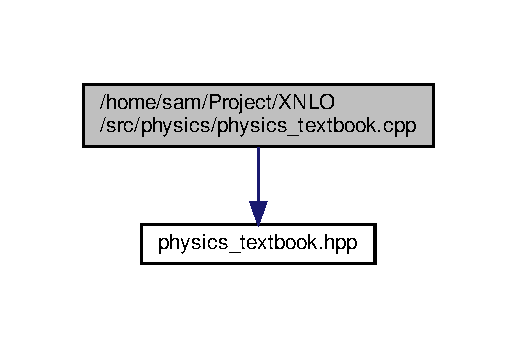
\includegraphics[width=210pt]{physics__textbook_8cpp__incl}
\end{center}
\end{figure}
\subsection*{Namespaces}
\begin{DoxyCompactItemize}
\item 
 \hyperlink{namespace_h_h_g_p}{H\+H\+GP}
\end{DoxyCompactItemize}

\hypertarget{physics__textbook_8hpp}{}\section{/home/sam/\+Project/\+X\+N\+L\+O/\+H\+H\+G\+P/src/physics\+\_\+textbook.hpp File Reference}
\label{physics__textbook_8hpp}\index{/home/sam/\+Project/\+X\+N\+L\+O/\+H\+H\+G\+P/src/physics\+\_\+textbook.\+hpp@{/home/sam/\+Project/\+X\+N\+L\+O/\+H\+H\+G\+P/src/physics\+\_\+textbook.\+hpp}}
This graph shows which files directly or indirectly include this file\+:\nopagebreak
\begin{figure}[H]
\begin{center}
\leavevmode
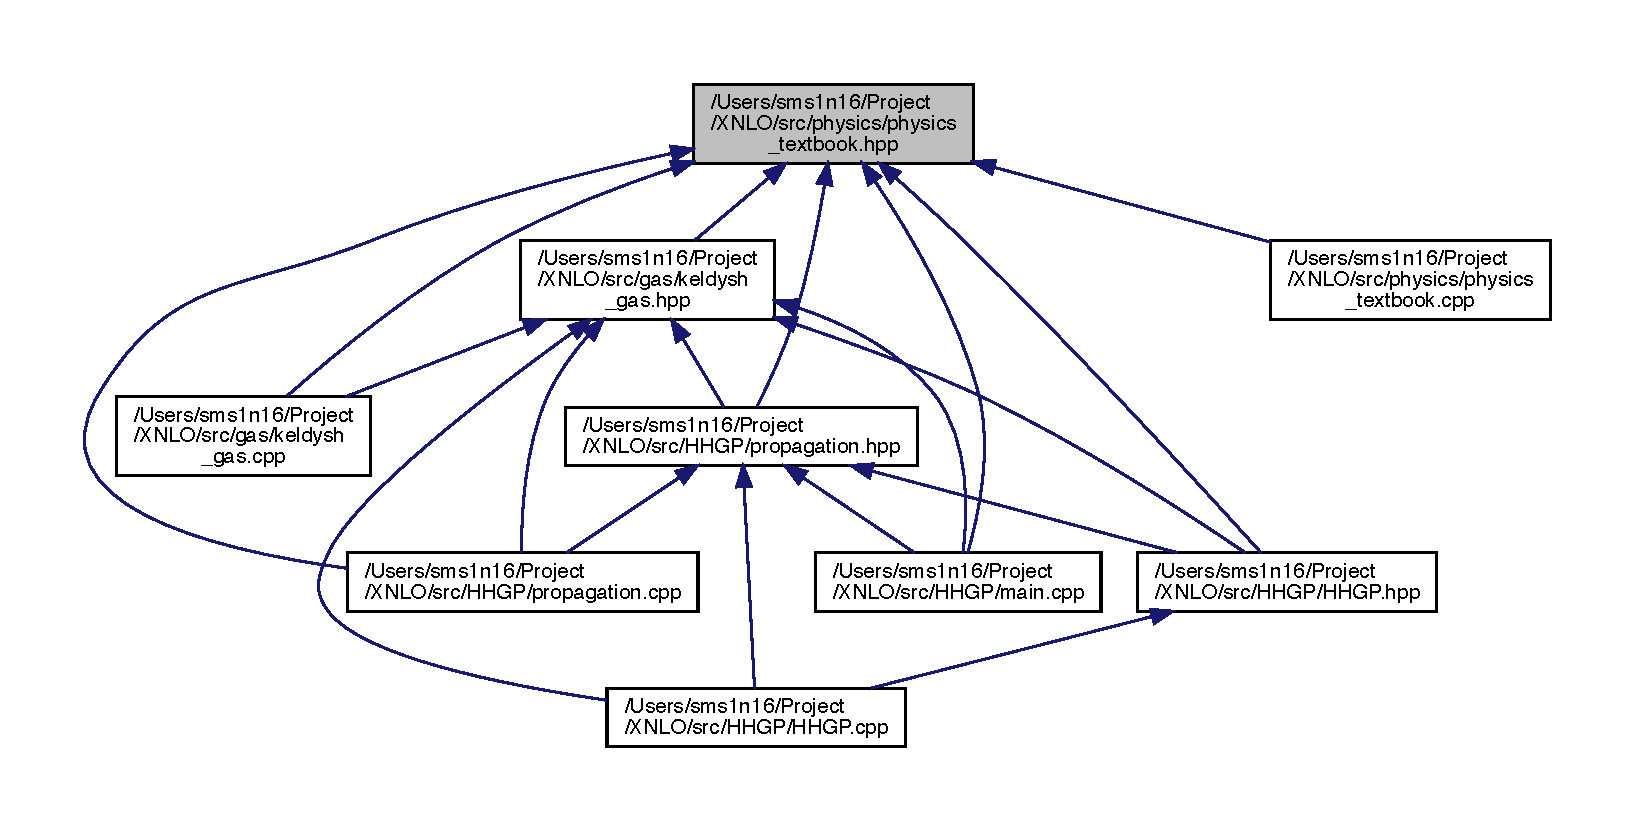
\includegraphics[width=350pt]{physics__textbook_8hpp__dep__incl}
\end{center}
\end{figure}
\subsection*{Classes}
\begin{DoxyCompactItemize}
\item 
class \hyperlink{classphysics__textbook}{physics\+\_\+textbook}
\end{DoxyCompactItemize}

\hypertarget{propagation_8cpp}{}\section{/home/sam/\+Project/\+X\+N\+L\+O/\+H\+H\+G\+P/src/propagation.cpp File Reference}
\label{propagation_8cpp}\index{/home/sam/\+Project/\+X\+N\+L\+O/\+H\+H\+G\+P/src/propagation.\+cpp@{/home/sam/\+Project/\+X\+N\+L\+O/\+H\+H\+G\+P/src/propagation.\+cpp}}
{\ttfamily \#include \char`\"{}propagation.\+hpp\char`\"{}}\newline
{\ttfamily \#include \char`\"{}../../src/keldysh\+\_\+gas.\+hpp\char`\"{}}\newline
{\ttfamily \#include \char`\"{}../../src/grid\+\_\+rkr.\+hpp\char`\"{}}\newline
{\ttfamily \#include \char`\"{}../../src/grid\+\_\+tw.\+hpp\char`\"{}}\newline
{\ttfamily \#include \char`\"{}../../src/\+D\+H\+T.\+hpp\char`\"{}}\newline
{\ttfamily \#include \char`\"{}../../src/physics\+\_\+textbook.\+hpp\char`\"{}}\newline
{\ttfamily \#include \char`\"{}../../src/maths\+\_\+textbook.\+hpp\char`\"{}}\newline
{\ttfamily \#include \char`\"{}Eigen/\+Dense\char`\"{}}\newline
{\ttfamily \#include $<$iostream$>$}\newline
{\ttfamily \#include \char`\"{}../../src/\+I\+O.\+hpp\char`\"{}}\newline
{\ttfamily \#include $<$complex$>$}\newline
Include dependency graph for propagation.\+cpp\+:
\nopagebreak
\begin{figure}[H]
\begin{center}
\leavevmode
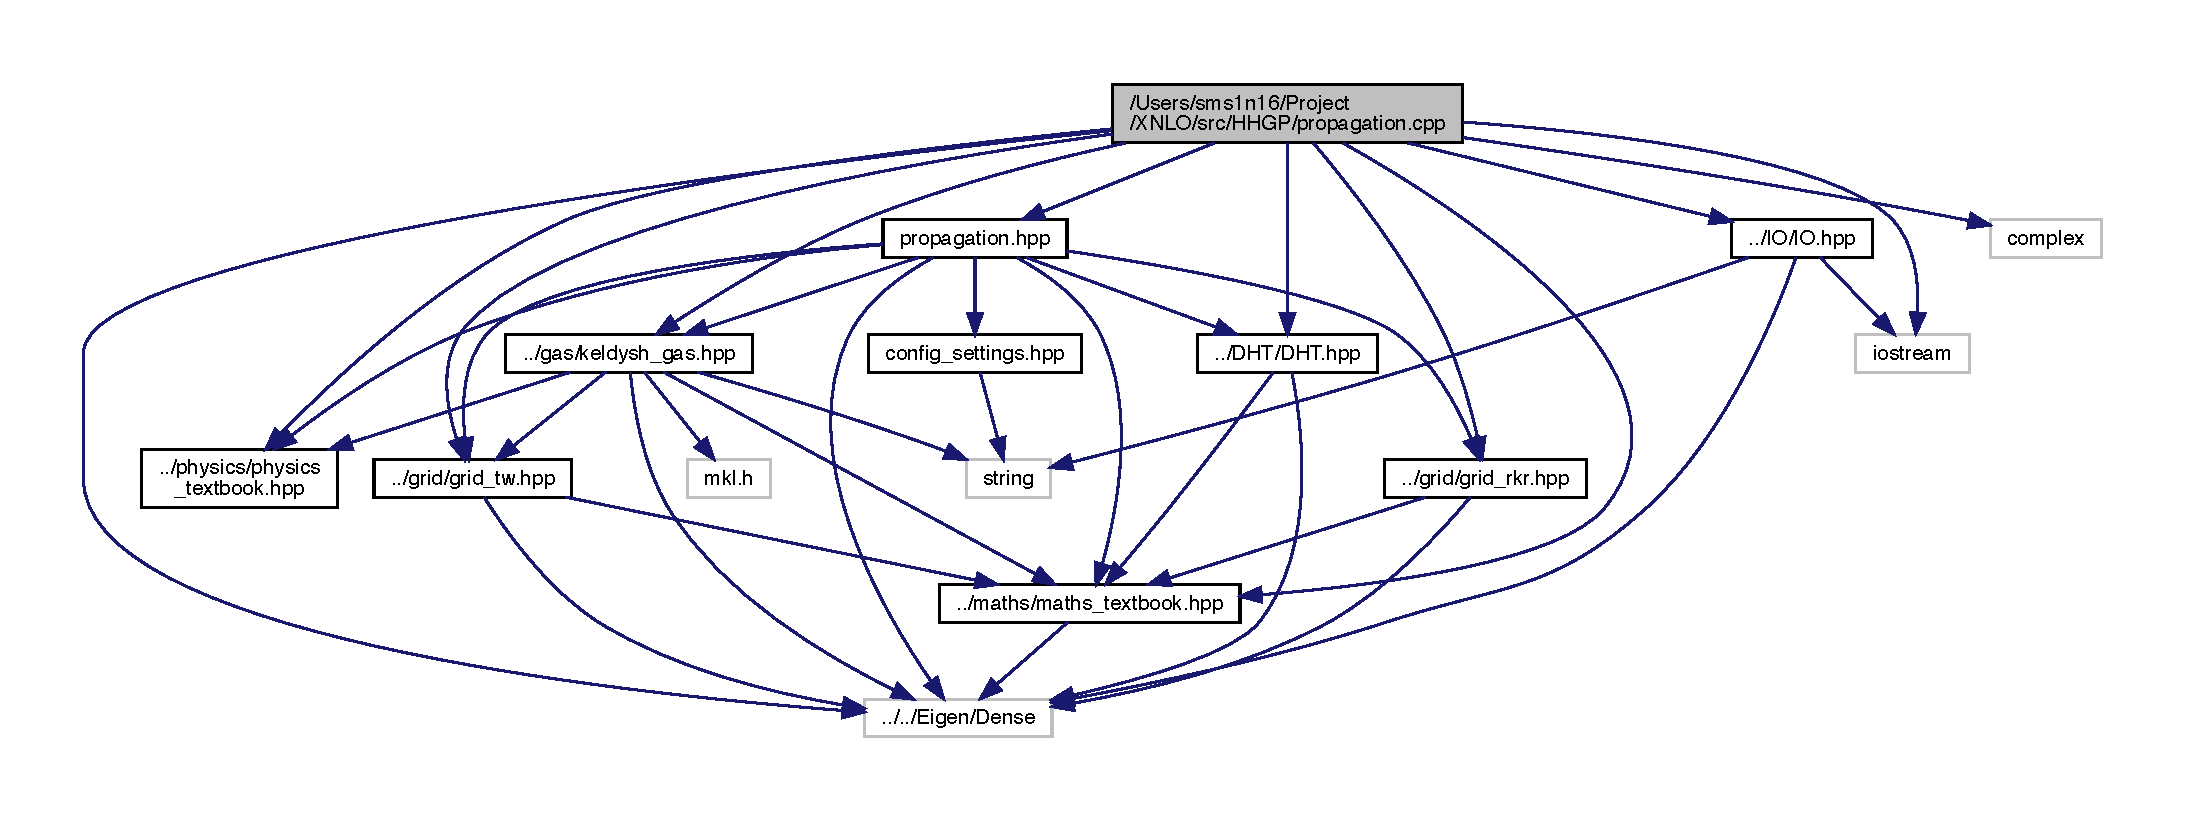
\includegraphics[width=350pt]{propagation_8cpp__incl}
\end{center}
\end{figure}

\hypertarget{propagation_8hpp}{}\section{/home/sam/\+Project/\+X\+N\+L\+O/src/\+H\+H\+G\+P/propagation.hpp File Reference}
\label{propagation_8hpp}\index{/home/sam/\+Project/\+X\+N\+L\+O/src/\+H\+H\+G\+P/propagation.\+hpp@{/home/sam/\+Project/\+X\+N\+L\+O/src/\+H\+H\+G\+P/propagation.\+hpp}}
{\ttfamily \#include \char`\"{}config\+\_\+settings.\+hpp\char`\"{}}\newline
{\ttfamily \#include \char`\"{}../gas/keldysh\+\_\+gas.\+hpp\char`\"{}}\newline
{\ttfamily \#include \char`\"{}../physics/physics\+\_\+textbook.\+hpp\char`\"{}}\newline
{\ttfamily \#include \char`\"{}../maths/maths\+\_\+textbook.\+hpp\char`\"{}}\newline
{\ttfamily \#include \char`\"{}../grid/grid\+\_\+rkr.\+hpp\char`\"{}}\newline
{\ttfamily \#include \char`\"{}../grid/grid\+\_\+tw.\+hpp\char`\"{}}\newline
{\ttfamily \#include \char`\"{}../\+D\+H\+T/\+D\+H\+T.\+hpp\char`\"{}}\newline
{\ttfamily \#include \char`\"{}../../\+Eigen/\+Dense\char`\"{}}\newline
Include dependency graph for propagation.\+hpp\+:\nopagebreak
\begin{figure}[H]
\begin{center}
\leavevmode
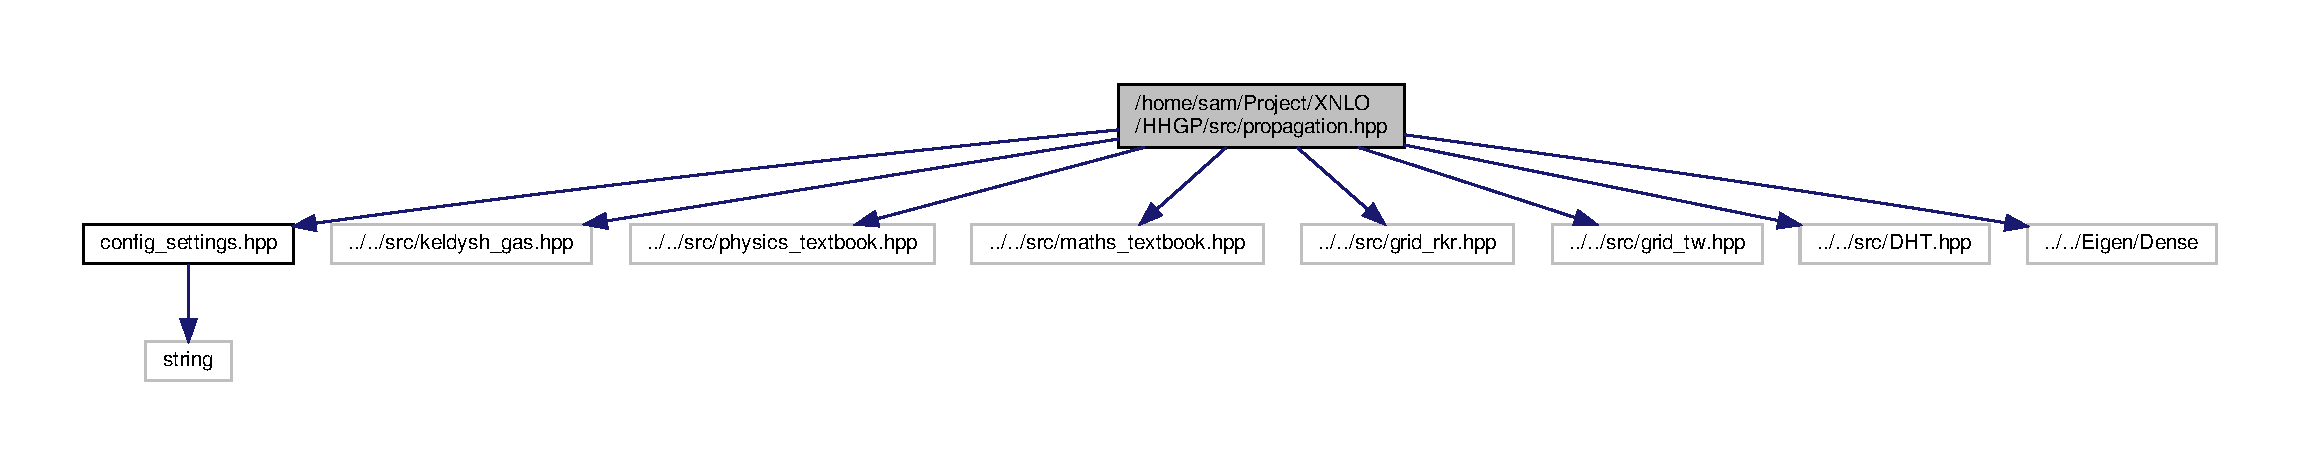
\includegraphics[width=350pt]{propagation_8hpp__incl}
\end{center}
\end{figure}
This graph shows which files directly or indirectly include this file\+:\nopagebreak
\begin{figure}[H]
\begin{center}
\leavevmode
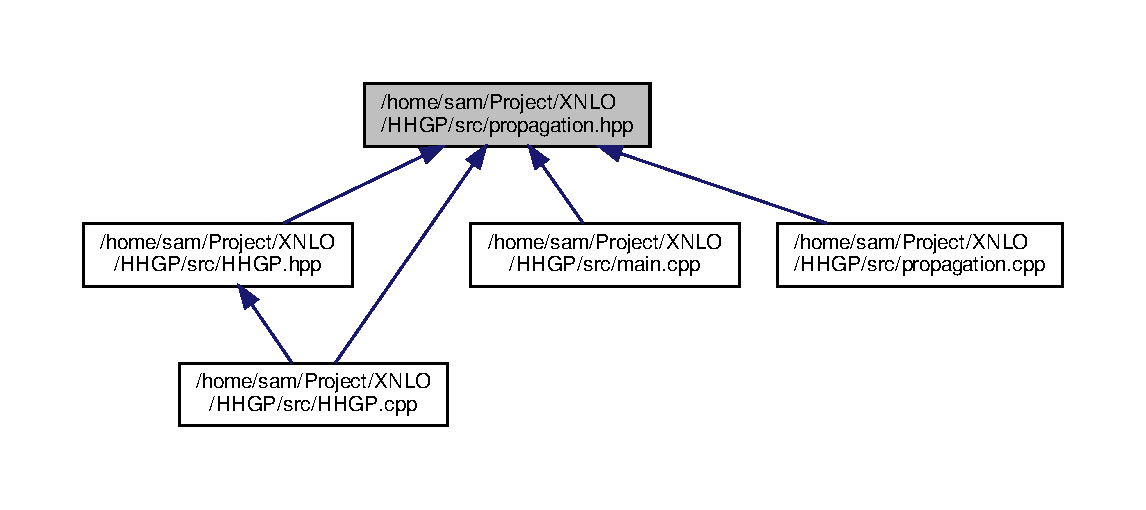
\includegraphics[width=350pt]{propagation_8hpp__dep__incl}
\end{center}
\end{figure}
\subsection*{Classes}
\begin{DoxyCompactItemize}
\item 
class \hyperlink{classpropagation}{propagation}
\end{DoxyCompactItemize}

\hypertarget{version_8hpp}{}\section{/home/sam/\+Project/\+X\+N\+L\+O/src/\+H\+H\+G\+P/version.hpp File Reference}
\label{version_8hpp}\index{/home/sam/\+Project/\+X\+N\+L\+O/src/\+H\+H\+G\+P/version.\+hpp@{/home/sam/\+Project/\+X\+N\+L\+O/src/\+H\+H\+G\+P/version.\+hpp}}
\subsection*{Macros}
\begin{DoxyCompactItemize}
\item 
\#define \hyperlink{version_8hpp_aac52b05128da45201ff8e39e39156b82}{\+\_\+\+V\+E\+R\+S\+I\+O\+N\+\_\+\+M\+A\+J\+OR}~2
\item 
\#define \hyperlink{version_8hpp_a1aac9829b460d4b1a2c8643fe7201524}{\+\_\+\+V\+E\+R\+S\+I\+O\+N\+\_\+\+M\+I\+N\+OR}~0
\item 
\#define \hyperlink{version_8hpp_abe78003459809bdd8d99f3b0b293b83f}{\+\_\+\+V\+E\+R\+S\+I\+O\+N\+\_\+\+S\+U\+B\+M\+I\+N\+OR}~0
\end{DoxyCompactItemize}


\subsection{Macro Definition Documentation}
\mbox{\Hypertarget{version_8hpp_aac52b05128da45201ff8e39e39156b82}\label{version_8hpp_aac52b05128da45201ff8e39e39156b82}} 
\index{version.\+hpp@{version.\+hpp}!\+\_\+\+V\+E\+R\+S\+I\+O\+N\+\_\+\+M\+A\+J\+OR@{\+\_\+\+V\+E\+R\+S\+I\+O\+N\+\_\+\+M\+A\+J\+OR}}
\index{\+\_\+\+V\+E\+R\+S\+I\+O\+N\+\_\+\+M\+A\+J\+OR@{\+\_\+\+V\+E\+R\+S\+I\+O\+N\+\_\+\+M\+A\+J\+OR}!version.\+hpp@{version.\+hpp}}
\subsubsection{\texorpdfstring{\+\_\+\+V\+E\+R\+S\+I\+O\+N\+\_\+\+M\+A\+J\+OR}{\_VERSION\_MAJOR}}
{\footnotesize\ttfamily \#define \+\_\+\+V\+E\+R\+S\+I\+O\+N\+\_\+\+M\+A\+J\+OR~2}

\mbox{\Hypertarget{version_8hpp_a1aac9829b460d4b1a2c8643fe7201524}\label{version_8hpp_a1aac9829b460d4b1a2c8643fe7201524}} 
\index{version.\+hpp@{version.\+hpp}!\+\_\+\+V\+E\+R\+S\+I\+O\+N\+\_\+\+M\+I\+N\+OR@{\+\_\+\+V\+E\+R\+S\+I\+O\+N\+\_\+\+M\+I\+N\+OR}}
\index{\+\_\+\+V\+E\+R\+S\+I\+O\+N\+\_\+\+M\+I\+N\+OR@{\+\_\+\+V\+E\+R\+S\+I\+O\+N\+\_\+\+M\+I\+N\+OR}!version.\+hpp@{version.\+hpp}}
\subsubsection{\texorpdfstring{\+\_\+\+V\+E\+R\+S\+I\+O\+N\+\_\+\+M\+I\+N\+OR}{\_VERSION\_MINOR}}
{\footnotesize\ttfamily \#define \+\_\+\+V\+E\+R\+S\+I\+O\+N\+\_\+\+M\+I\+N\+OR~0}

\mbox{\Hypertarget{version_8hpp_abe78003459809bdd8d99f3b0b293b83f}\label{version_8hpp_abe78003459809bdd8d99f3b0b293b83f}} 
\index{version.\+hpp@{version.\+hpp}!\+\_\+\+V\+E\+R\+S\+I\+O\+N\+\_\+\+S\+U\+B\+M\+I\+N\+OR@{\+\_\+\+V\+E\+R\+S\+I\+O\+N\+\_\+\+S\+U\+B\+M\+I\+N\+OR}}
\index{\+\_\+\+V\+E\+R\+S\+I\+O\+N\+\_\+\+S\+U\+B\+M\+I\+N\+OR@{\+\_\+\+V\+E\+R\+S\+I\+O\+N\+\_\+\+S\+U\+B\+M\+I\+N\+OR}!version.\+hpp@{version.\+hpp}}
\subsubsection{\texorpdfstring{\+\_\+\+V\+E\+R\+S\+I\+O\+N\+\_\+\+S\+U\+B\+M\+I\+N\+OR}{\_VERSION\_SUBMINOR}}
{\footnotesize\ttfamily \#define \+\_\+\+V\+E\+R\+S\+I\+O\+N\+\_\+\+S\+U\+B\+M\+I\+N\+OR~0}


%--- End generated contents ---

% Index
\backmatter
\newpage
\phantomsection
\clearemptydoublepage
\addcontentsline{toc}{chapter}{Index}
\printindex

\end{document}
